\section{Background}

In this chapter we review: existing software abstractions for mesh computations, common strategies for optimising performance, and mesh-specific optimisations.

\subsection{Existing software abstractions}

\subsubsection{Stencil languages}
\label{sec:stencillang}

% can be classified according to whether or not they know about the mesh - makes describing connectivity clearer,
% but requires a hand-written mesh implementation lacking features and hard to maintain

Given the ubiquity of stencil operations in simulations, a number of libraries exist providing convenient interfaces for stencil applications.

% they are largely all inspired by the following pieces of info:
% - a mesh can be considered as sets of entities
% - one loops over a set, collects adjacent data, then calls some local kernel
% - the local kernel may be written in the same language as the stencil language, but it needn't be

Ebb, Simit and Liszt follow the approach of providing a domain-specific language for the expression of stencil problems...
They all provide high performance execution on GPUs as well as CPUs.

% i don't think simit works on MPI

OP2 is another approach~\cite{mudaligeOP2ActiveLibrary2012,mudaligeDesignInitialPerformance2013}.
Rather than using a domain-specific language, OP2 provides a simple API to the user for specifying the problem.
The key entities in the OP2 data model are: sets, data on sets, mappings between sets, and operations applied over these sets.
Having provided these inputs, the OP2 compiler is then called and transforms to source code to a high performance implementation of the traversal for a specific architecture.

% then PyOP2
% describe libCEED - main benefit is that it is fast.

% it is noteworthy that Ebb, Simit, Liszt have custom implementations of unstructured meshes.
% whereas (Py)OP2 and libCEED have an abstraction that does not specifically include a mesh.
% the latter is favourable as one can reuse existing solutions to other mesh problems like
% refinement, adaptivity, I/O, decomposition...
% however, lack of topological information can make code unreadable, hard to write as
% topological info is lost, e.g. composability is not really possible.

% this leads very nicely into discussion of DMPlex
% note: we don't have a nice solution to orientations yet - but no one does

Another library for the application of stencil operations, specifically high-order matrix-free kernels for the \gls{fem}, is libCEED.
% libceed - actually offloaded to PETSc for element restriction (the bit PyOP2 does)
% it's nice that libCEED and PyOP2 use DMPlex as the burden of other mesh operations (e.g. distribution, I/O, refinement) are very non-trivial

PyOP2 is a domain-specific language for expressing computations over unstructured meshes.
It is the direct precursor, and inspiration for, \projectname.

It distinguishes itself from OP2, a library depending on the same abstractions, by using run-time code generation instead of static analysis and transformation of the source code.

PyOP2's mesh abstraction is formed out of the following main components:

% \begin{itemize}
%   \item \mintinline{python}{set}
% \end{itemize}

In PyOP2, data is defined on \textit{sets} and these are related to one another using \textit{mappings}.
Importantly, this abstraction does not contain any concept of the underlying mesh and instead all of the required information is encoded in the maps.

  Computations over the mesh are expressed as the execution of some local kernel over all entities of some iteration set via a construct called a parallel loop, or \textit{parloop}.
  The kernel is written using Loopy, a library for expressing array-based computations in a platform-generic language~\cite{klocknerLooPyTransformationbased2014}.
  This intermediate representation allows for interplay between the local kernels enabling optimisations such as inter-element vectorisation~\cite{sunStudyVectorizationMatrixfree2020}.

  At present, PyOP2 only works on distributed memory, CPU-only systems (although some work has been done to permit execution on GPUs~\cite{fenics2021-kulkarni}).
  During the execution of a parloop, each rank works independently on some partition of the mesh.
  To avoid excessive communication between ranks, each rank has a narrow \textit{halo} region that overlaps with neighbouring ranks that is executed redundantly.
  The halos are split into \textit{owned}, \textit{exec}, and \textit{non-exec} regions to indicate the data's origin and the communication direction between the neighbouring processes.


% Liszt, Simit - notably associates data information with topological entities

\subsubsection{Mesh representations}

% need to emphasise the difference between nodes and points

In software, a mesh is typically represented by a collection of sets of entities (e.g. cells or faces), coupled with adjacency relations between these sets.
Possible abstractions capturing this behaviour include databases (ebb, moab) or hypergraphs (simit).
In this work we focus on DMPlex, the unstructured mesh abstraction used in PETSc.
In contrast with Ebb, Simit or Liszt, DMPlex is a more general purpose mesh abstraction and so has a more substantial feature set.

% parallel partioning, adaptation, I/O, AMR...

In DMPlex, the mesh is represented as a \textit{CW-complex}, an object from algebraic topology that describes some topological space.
In such a complex, all topological entities (e.g. cells, vertices) are simply referred to as \textit{points} and the connectivity of the mesh can be expressed as the edges of a \gls{dag} with the vertices being the points of the mesh.
More specifically, the points and relations form a \gls{poset} such that the mesh can be visualised using a Hasse diagram (Figure~\ref{fig:hasse_diagram}).

It is important to note that DMPlex works for arbitrary dimension.

\begin{figure}
  \begin{subfigure}{0.45\textwidth}
    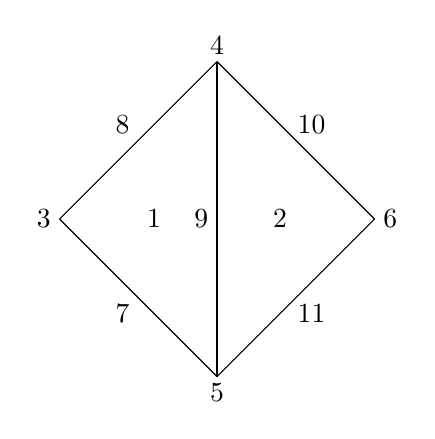
\begin{tikzpicture}
      \draw (0,2) -- (2,0);
      \draw (0,2) -- (2,4);
      \draw (2,0) -- (2,4);
      \draw (2,0) -- (4,2);
      \draw (2,4) -- (4,2);

      \node[at={(1,2)}, xshift=.2cm] {1};
      \node[at={(3,2)}, xshift=-.2cm] {2};
      \node[at={(0,2)}, xshift=-.2cm] {3};
      \node[at={(2,4)}, yshift=.2cm] {4};
      \node[at={(2,0)}, yshift=-.2cm] {5};
      \node[at={(4,2)}, xshift=.2cm] {6};
      \node[at={(1,1)}, xshift=-.2cm, yshift=-.2cm] {7};
      \node[at={(1,3)}, xshift=-.2cm, yshift=.2cm] {8};
      \node[at={(2,2)}, xshift=-.2cm] {9};
      \node[at={(3,3)}, xshift=.2cm, yshift=.2cm] {10};
      \node[at={(3,1)}, xshift=.2cm, yshift=-.2cm] {11};
    \end{tikzpicture}
  \end{subfigure}
  %
  \begin{subfigure}{0.45\textwidth}
    \centering
    \begin{tikzpicture}
      \basichasse
    \end{tikzpicture}
  \end{subfigure}

  \caption{...}
  \label{fig:hasse_diagram}
\end{figure}

\begin{figure}
  \centering
  \begin{subfigure}{0.45\textwidth}
    \centering
    \begin{tikzpicture}
      \basichasse
      \drawpolygon 7,9;
      \draw [dashed] (1) circle [radius=15pt];
    \end{tikzpicture}
    \caption{$cone(1)$}
  \end{subfigure}
  \begin{subfigure}{0.45\textwidth}
    \centering
    \begin{tikzpicture}
      \basichasse
      \drawpolygon 1,2;
      \draw [dashed] (9) circle [radius=15pt];
    \end{tikzpicture}
    \caption{$supp(9)$}
  \end{subfigure}
  \begin{subfigure}{0.45\textwidth}
    \centering
    \begin{tikzpicture}
      \basichasse
      \drawpolygon 1,7,3,5,9;
    \end{tikzpicture}
    \caption{$cl(1)$}
  \end{subfigure}
  \begin{subfigure}{0.45\textwidth}
    \centering
    \begin{tikzpicture}
      \basichasse
      \drawpolygon 4,10,2,1,8;
    \end{tikzpicture}
    \caption{$star(4)$}
  \end{subfigure}

  \caption{...}
  \label{fig:plex_restrictions}
\end{figure}


Stencil queries are natural to express at this level.
For instance, the classical finite element request of ``give me all of the \glspl{dof} that have local support" is simply expressed as the closure of a given cell.
Another example useful for finite volume calculations: ``what are my neighbouring cells?" is supp(cone(c)).
One can also do clever patch things.

With DMPlex, parallel vectors are created by associating a DMPlex mesh with a \clang{PetscSection}.
A \clang{PetscSection} is a simple object that tabulates offsets such that entries in an array may be addressed.

\subsection{Methods for performance optimisation}

In this section we review some of the common bottlenecks in massively parallel simulation codes, and describe some general ways for quantifying and improving performance.
In particular we focus on challenges for maximising parallel efficiency and the importance of the roofline model for choosing appropriate optimisations.
The aim is to motivate design choices made in \pyop3.

\subsubsection{Optimisation methodology}

Premature optimisation is a classic trap software developers fall into when they attempt to accelerate their codes.
It is surprisingly easy to find oneself making assumptions about the locations and causes of bottlenecks, and then wasting a considerable amount of time on optimising code that only constitutes a small fraction of the overall wall-clock time.
To avoid this scenario, developers should follow the steps below:

\begin{enumerate}
  \item
    \textbf{Find a realistic problem to try and accelerate.}

    Performance optimisation is often guided by toy problems that are simple to write and debug.
    Such problems, though, may end up having significantly different performance characteristics from a realistic simulation that a user would actually run.
    This can lead to premature optimisation as the wrong hotspots will be targeted.
    As a relevant example, one could work hard to optimise data movement for the application of low-order matrix-free stencils since the code will be memory-bound (see section~\ref{sec:background_perf_flops}) and so data movement would be the predominant cost.
    However, matrix-free methods are usually only applied at high-order~\cite{brownPerformancePortableSolid2022}, at which point the code will be compute-bound and the hotspots will be different.
  \item
    \textbf{Identify the hotspots.}
    \dots
    % flamegraph
  \item
    \textbf{Create a performance model.}
    \dots
    % roofline, think about message passing if needed
  \item
    \textbf{Optimise the code.}
    \dots
    % prioritise algorithmic changes over low-level optimisations as these can change convergence stuff
    % ref TAS spectrum?
  \item
    \textbf{Repeat?}
    \dots
    % are we at the fundamental limit of the machine?
    % is our scaling 'good enough'
\end{enumerate}

\subsubsection{Achieving parallel efficiency}
\label{sec:background_perf_efficiency}

In order to run massive simulations, codes must be able to exploit the massive amounts of parallelism afforded to them by modern supercomputers.
With the building of ever larger and more parallel machines (especially since we are at the ``dawn of exascale''), this is becoming both more important to get right and more challenging to do so.

To quantify a code's effectiveness in parallel, one typically measures its \textit{parallel efficiency} under either \textit{strong-} or \textit{weak-scaling}:

\begin{paragraph}{Strong-scaling}
A strong-scaling investigation would solve the same problem but on an increasing number of processors and measure the time-to-solution.
Perfect efficiency (unity) would be achieved if the time-to-solution on $p$ processors was $p$ times smaller than the time-to-solution for a single process.
If strong-scaling efficiency is poor, this suggests that there are sizeable portions of the code that are getting run in serial on each process, rather than being divided up.
A code would be considered to have `good' strong-scaling if it retained high efficiency (e.g. 80\%) at small problem sizes (e.g. 5000 \glspl{dof} per process for \gls{fem}).
\end{paragraph}

\begin{paragraph}{Weak-scaling}
Weak-scaling differs from strong-scaling by, rather than measuring the decrease in time-to-solution for a problem of fixed size, recording the time-to-solution for a range of problem sizes where the size of the problem scales linearly with the number of processors.
In this case, perfect efficiency is achieved if the time-to-solution remains fixed.
If a code has poor weak-scaling, this suggests that there are algorithmic problems regarding how the problem is distributed among processors.
For example, a parallel algorithm that required frequent all-to-all broadcast messages would have poor weak-scaling because this would increase in cost with the number of processors.
For a code to have `good' weak-scaling, it would need to have a high efficiency (e.g. 80\%) even when run on very large clusters.
\end{paragraph}

\vspace{1em}

Taken together, these two metrics provide a relatively good indicator as to the suitability of a code for running on massively parallel computers, which is naturally essential for simulation codes to be effective.
More informative measures of performance that take into account things such as convergence rates also exist~\cite{changComparativeStudyFinite2018}, but we eschew such measures here because they fall under the remit of the design of the stencil itself, rather than the stencil \textit{iteration}, which is the focus for this work.

\subsubsection{Maximising floating-point throughput}
\label{sec:background_perf_flops}

Once we have a code that scales well, the next step is to optimise performance for a single process.
In order to do this, one should first profile the code and compare its performance to the theoretical limits of the hardware.
Doing this provides both a good termination criterion for the optimisation process (you can't go faster than the hardware!), and also guides the developer as to what the performance bottlenecks might be and thus which optimisations might be usefully applied.

As a first step, one should profile the performance-critical kernels in the application to determine their floating-point throughput (the higher the better) and their \gls{ai}.
Arithmetic intensity is a ratio of the number of \glspl{flop} performed per byte of memory accessed.
To simplify, a kernel with low arithmetic intensity reads a lot of data from memory but the processor does not need to perform many calculations, and a kernel with high arithmetic intensity performs a lot of calculations per byte of memory accessed.
An example of a kernel with low \gls{ai} would be \mintinline{c}{z[i] = x[i] + y[i];}; 1 \gls{flop} (addition) is performed for every 3 data accesses (2 reads and 1 write).
Assuming that \mintinline{c}{x}, \mintinline{c}{y} and \mintinline{c}{z} are 8 bytes each, this gives this operation an \gls{ai} of $1/24$.
In contrast, a kernel with a high \gls{ai} might include operations of the form \mintinline{c}{y[i] = sqrt(x[i]);}.
Operations such as square roots and division typically require a large number of \glspl{flop}, increasing the \gls{ai}.

The key insight that \gls{ai} gives us is that some applications are limited by the rate at which \textit{memory is accessed}, and some applications are limited by the rate at which \textit{chips perform \glspl{flop}}.
These are typically referred to as \textit{memory-bound} and \textit{compute-bound} respectively.
It is worthwhile to note that there is trend in modern chips for floating-point throughput to increase at a faster rate than memory bandwidth, and so more and more codes are becoming memory-bound.

\begin{figure}
  %% Creator: Matplotlib, PGF backend
%%
%% To include the figure in your LaTeX document, write
%%   \input{<filename>.pgf}
%%
%% Make sure the required packages are loaded in your preamble
%%   \usepackage{pgf}
%%
%% Also ensure that all the required font packages are loaded; for instance,
%% the lmodern package is sometimes necessary when using math font.
%%   \usepackage{lmodern}
%%
%% Figures using additional raster images can only be included by \input if
%% they are in the same directory as the main LaTeX file. For loading figures
%% from other directories you can use the `import` package
%%   \usepackage{import}
%%
%% and then include the figures with
%%   \import{<path to file>}{<filename>.pgf}
%%
%% Matplotlib used the following preamble
%%   
%%   \usepackage{fontspec}
%%   \setmainfont{DejaVuSerif.ttf}[Path=\detokenize{/home/connor/Code/late-stage-review/venv/lib/python3.10/site-packages/matplotlib/mpl-data/fonts/ttf/}]
%%   \setsansfont{DejaVuSans.ttf}[Path=\detokenize{/home/connor/Code/late-stage-review/venv/lib/python3.10/site-packages/matplotlib/mpl-data/fonts/ttf/}]
%%   \setmonofont{DejaVuSansMono.ttf}[Path=\detokenize{/home/connor/Code/late-stage-review/venv/lib/python3.10/site-packages/matplotlib/mpl-data/fonts/ttf/}]
%%   \makeatletter\@ifpackageloaded{underscore}{}{\usepackage[strings]{underscore}}\makeatother
%%
\begingroup%
\makeatletter%
\begin{pgfpicture}%
\pgfpathrectangle{\pgfpointorigin}{\pgfqpoint{4.541667in}{3.638889in}}%
\pgfusepath{use as bounding box, clip}%
\begin{pgfscope}%
\pgfsetbuttcap%
\pgfsetmiterjoin%
\definecolor{currentfill}{rgb}{1.000000,1.000000,1.000000}%
\pgfsetfillcolor{currentfill}%
\pgfsetlinewidth{0.000000pt}%
\definecolor{currentstroke}{rgb}{1.000000,1.000000,1.000000}%
\pgfsetstrokecolor{currentstroke}%
\pgfsetdash{}{0pt}%
\pgfpathmoveto{\pgfqpoint{0.000000in}{0.000000in}}%
\pgfpathlineto{\pgfqpoint{4.541667in}{0.000000in}}%
\pgfpathlineto{\pgfqpoint{4.541667in}{3.638889in}}%
\pgfpathlineto{\pgfqpoint{0.000000in}{3.638889in}}%
\pgfpathlineto{\pgfqpoint{0.000000in}{0.000000in}}%
\pgfpathclose%
\pgfusepath{fill}%
\end{pgfscope}%
\begin{pgfscope}%
\pgfsetbuttcap%
\pgfsetmiterjoin%
\definecolor{currentfill}{rgb}{1.000000,1.000000,1.000000}%
\pgfsetfillcolor{currentfill}%
\pgfsetlinewidth{0.000000pt}%
\definecolor{currentstroke}{rgb}{0.000000,0.000000,0.000000}%
\pgfsetstrokecolor{currentstroke}%
\pgfsetstrokeopacity{0.000000}%
\pgfsetdash{}{0pt}%
\pgfpathmoveto{\pgfqpoint{0.567708in}{0.400278in}}%
\pgfpathlineto{\pgfqpoint{4.087500in}{0.400278in}}%
\pgfpathlineto{\pgfqpoint{4.087500in}{3.202222in}}%
\pgfpathlineto{\pgfqpoint{0.567708in}{3.202222in}}%
\pgfpathlineto{\pgfqpoint{0.567708in}{0.400278in}}%
\pgfpathclose%
\pgfusepath{fill}%
\end{pgfscope}%
\begin{pgfscope}%
\pgfpathrectangle{\pgfqpoint{0.567708in}{0.400278in}}{\pgfqpoint{3.519792in}{2.801944in}}%
\pgfusepath{clip}%
\pgfsetbuttcap%
\pgfsetroundjoin%
\definecolor{currentfill}{rgb}{1.000000,0.000000,0.000000}%
\pgfsetfillcolor{currentfill}%
\pgfsetlinewidth{1.003750pt}%
\definecolor{currentstroke}{rgb}{1.000000,0.000000,0.000000}%
\pgfsetstrokecolor{currentstroke}%
\pgfsetdash{}{0pt}%
\pgfsys@defobject{currentmarker}{\pgfqpoint{-0.041667in}{-0.041667in}}{\pgfqpoint{0.041667in}{0.041667in}}{%
\pgfpathmoveto{\pgfqpoint{0.000000in}{-0.041667in}}%
\pgfpathcurveto{\pgfqpoint{0.011050in}{-0.041667in}}{\pgfqpoint{0.021649in}{-0.037276in}}{\pgfqpoint{0.029463in}{-0.029463in}}%
\pgfpathcurveto{\pgfqpoint{0.037276in}{-0.021649in}}{\pgfqpoint{0.041667in}{-0.011050in}}{\pgfqpoint{0.041667in}{0.000000in}}%
\pgfpathcurveto{\pgfqpoint{0.041667in}{0.011050in}}{\pgfqpoint{0.037276in}{0.021649in}}{\pgfqpoint{0.029463in}{0.029463in}}%
\pgfpathcurveto{\pgfqpoint{0.021649in}{0.037276in}}{\pgfqpoint{0.011050in}{0.041667in}}{\pgfqpoint{0.000000in}{0.041667in}}%
\pgfpathcurveto{\pgfqpoint{-0.011050in}{0.041667in}}{\pgfqpoint{-0.021649in}{0.037276in}}{\pgfqpoint{-0.029463in}{0.029463in}}%
\pgfpathcurveto{\pgfqpoint{-0.037276in}{0.021649in}}{\pgfqpoint{-0.041667in}{0.011050in}}{\pgfqpoint{-0.041667in}{0.000000in}}%
\pgfpathcurveto{\pgfqpoint{-0.041667in}{-0.011050in}}{\pgfqpoint{-0.037276in}{-0.021649in}}{\pgfqpoint{-0.029463in}{-0.029463in}}%
\pgfpathcurveto{\pgfqpoint{-0.021649in}{-0.037276in}}{\pgfqpoint{-0.011050in}{-0.041667in}}{\pgfqpoint{0.000000in}{-0.041667in}}%
\pgfpathlineto{\pgfqpoint{0.000000in}{-0.041667in}}%
\pgfpathclose%
\pgfusepath{stroke,fill}%
}%
\begin{pgfscope}%
\pgfsys@transformshift{1.082402in}{0.902053in}%
\pgfsys@useobject{currentmarker}{}%
\end{pgfscope}%
\end{pgfscope}%
\begin{pgfscope}%
\pgfpathrectangle{\pgfqpoint{0.567708in}{0.400278in}}{\pgfqpoint{3.519792in}{2.801944in}}%
\pgfusepath{clip}%
\pgfsetbuttcap%
\pgfsetroundjoin%
\definecolor{currentfill}{rgb}{1.000000,0.000000,0.000000}%
\pgfsetfillcolor{currentfill}%
\pgfsetlinewidth{1.003750pt}%
\definecolor{currentstroke}{rgb}{1.000000,0.000000,0.000000}%
\pgfsetstrokecolor{currentstroke}%
\pgfsetdash{}{0pt}%
\pgfsys@defobject{currentmarker}{\pgfqpoint{-0.041667in}{-0.041667in}}{\pgfqpoint{0.041667in}{0.041667in}}{%
\pgfpathmoveto{\pgfqpoint{0.000000in}{-0.041667in}}%
\pgfpathcurveto{\pgfqpoint{0.011050in}{-0.041667in}}{\pgfqpoint{0.021649in}{-0.037276in}}{\pgfqpoint{0.029463in}{-0.029463in}}%
\pgfpathcurveto{\pgfqpoint{0.037276in}{-0.021649in}}{\pgfqpoint{0.041667in}{-0.011050in}}{\pgfqpoint{0.041667in}{0.000000in}}%
\pgfpathcurveto{\pgfqpoint{0.041667in}{0.011050in}}{\pgfqpoint{0.037276in}{0.021649in}}{\pgfqpoint{0.029463in}{0.029463in}}%
\pgfpathcurveto{\pgfqpoint{0.021649in}{0.037276in}}{\pgfqpoint{0.011050in}{0.041667in}}{\pgfqpoint{0.000000in}{0.041667in}}%
\pgfpathcurveto{\pgfqpoint{-0.011050in}{0.041667in}}{\pgfqpoint{-0.021649in}{0.037276in}}{\pgfqpoint{-0.029463in}{0.029463in}}%
\pgfpathcurveto{\pgfqpoint{-0.037276in}{0.021649in}}{\pgfqpoint{-0.041667in}{0.011050in}}{\pgfqpoint{-0.041667in}{0.000000in}}%
\pgfpathcurveto{\pgfqpoint{-0.041667in}{-0.011050in}}{\pgfqpoint{-0.037276in}{-0.021649in}}{\pgfqpoint{-0.029463in}{-0.029463in}}%
\pgfpathcurveto{\pgfqpoint{-0.021649in}{-0.037276in}}{\pgfqpoint{-0.011050in}{-0.041667in}}{\pgfqpoint{0.000000in}{-0.041667in}}%
\pgfpathlineto{\pgfqpoint{0.000000in}{-0.041667in}}%
\pgfpathclose%
\pgfusepath{stroke,fill}%
}%
\begin{pgfscope}%
\pgfsys@transformshift{3.085801in}{1.187726in}%
\pgfsys@useobject{currentmarker}{}%
\end{pgfscope}%
\end{pgfscope}%
\begin{pgfscope}%
\pgfpathrectangle{\pgfqpoint{0.567708in}{0.400278in}}{\pgfqpoint{3.519792in}{2.801944in}}%
\pgfusepath{clip}%
\pgfsetbuttcap%
\pgfsetroundjoin%
\definecolor{currentfill}{rgb}{1.000000,0.000000,0.000000}%
\pgfsetfillcolor{currentfill}%
\pgfsetlinewidth{1.003750pt}%
\definecolor{currentstroke}{rgb}{1.000000,0.000000,0.000000}%
\pgfsetstrokecolor{currentstroke}%
\pgfsetdash{}{0pt}%
\pgfsys@defobject{currentmarker}{\pgfqpoint{-0.041667in}{-0.041667in}}{\pgfqpoint{0.041667in}{0.041667in}}{%
\pgfpathmoveto{\pgfqpoint{0.000000in}{-0.041667in}}%
\pgfpathcurveto{\pgfqpoint{0.011050in}{-0.041667in}}{\pgfqpoint{0.021649in}{-0.037276in}}{\pgfqpoint{0.029463in}{-0.029463in}}%
\pgfpathcurveto{\pgfqpoint{0.037276in}{-0.021649in}}{\pgfqpoint{0.041667in}{-0.011050in}}{\pgfqpoint{0.041667in}{0.000000in}}%
\pgfpathcurveto{\pgfqpoint{0.041667in}{0.011050in}}{\pgfqpoint{0.037276in}{0.021649in}}{\pgfqpoint{0.029463in}{0.029463in}}%
\pgfpathcurveto{\pgfqpoint{0.021649in}{0.037276in}}{\pgfqpoint{0.011050in}{0.041667in}}{\pgfqpoint{0.000000in}{0.041667in}}%
\pgfpathcurveto{\pgfqpoint{-0.011050in}{0.041667in}}{\pgfqpoint{-0.021649in}{0.037276in}}{\pgfqpoint{-0.029463in}{0.029463in}}%
\pgfpathcurveto{\pgfqpoint{-0.037276in}{0.021649in}}{\pgfqpoint{-0.041667in}{0.011050in}}{\pgfqpoint{-0.041667in}{0.000000in}}%
\pgfpathcurveto{\pgfqpoint{-0.041667in}{-0.011050in}}{\pgfqpoint{-0.037276in}{-0.021649in}}{\pgfqpoint{-0.029463in}{-0.029463in}}%
\pgfpathcurveto{\pgfqpoint{-0.021649in}{-0.037276in}}{\pgfqpoint{-0.011050in}{-0.041667in}}{\pgfqpoint{0.000000in}{-0.041667in}}%
\pgfpathlineto{\pgfqpoint{0.000000in}{-0.041667in}}%
\pgfpathclose%
\pgfusepath{stroke,fill}%
}%
\begin{pgfscope}%
\pgfsys@transformshift{3.667269in}{2.521065in}%
\pgfsys@useobject{currentmarker}{}%
\end{pgfscope}%
\end{pgfscope}%
\begin{pgfscope}%
\pgfsetbuttcap%
\pgfsetroundjoin%
\definecolor{currentfill}{rgb}{0.000000,0.000000,0.000000}%
\pgfsetfillcolor{currentfill}%
\pgfsetlinewidth{0.803000pt}%
\definecolor{currentstroke}{rgb}{0.000000,0.000000,0.000000}%
\pgfsetstrokecolor{currentstroke}%
\pgfsetdash{}{0pt}%
\pgfsys@defobject{currentmarker}{\pgfqpoint{0.000000in}{-0.048611in}}{\pgfqpoint{0.000000in}{0.000000in}}{%
\pgfpathmoveto{\pgfqpoint{0.000000in}{0.000000in}}%
\pgfpathlineto{\pgfqpoint{0.000000in}{-0.048611in}}%
\pgfusepath{stroke,fill}%
}%
\begin{pgfscope}%
\pgfsys@transformshift{0.590121in}{0.400278in}%
\pgfsys@useobject{currentmarker}{}%
\end{pgfscope}%
\end{pgfscope}%
\begin{pgfscope}%
\pgfsetbuttcap%
\pgfsetroundjoin%
\definecolor{currentfill}{rgb}{0.000000,0.000000,0.000000}%
\pgfsetfillcolor{currentfill}%
\pgfsetlinewidth{0.803000pt}%
\definecolor{currentstroke}{rgb}{0.000000,0.000000,0.000000}%
\pgfsetstrokecolor{currentstroke}%
\pgfsetdash{}{0pt}%
\pgfsys@defobject{currentmarker}{\pgfqpoint{0.000000in}{-0.048611in}}{\pgfqpoint{0.000000in}{0.000000in}}{%
\pgfpathmoveto{\pgfqpoint{0.000000in}{0.000000in}}%
\pgfpathlineto{\pgfqpoint{0.000000in}{-0.048611in}}%
\pgfusepath{stroke,fill}%
}%
\begin{pgfscope}%
\pgfsys@transformshift{1.422014in}{0.400278in}%
\pgfsys@useobject{currentmarker}{}%
\end{pgfscope}%
\end{pgfscope}%
\begin{pgfscope}%
\pgfsetbuttcap%
\pgfsetroundjoin%
\definecolor{currentfill}{rgb}{0.000000,0.000000,0.000000}%
\pgfsetfillcolor{currentfill}%
\pgfsetlinewidth{0.803000pt}%
\definecolor{currentstroke}{rgb}{0.000000,0.000000,0.000000}%
\pgfsetstrokecolor{currentstroke}%
\pgfsetdash{}{0pt}%
\pgfsys@defobject{currentmarker}{\pgfqpoint{0.000000in}{-0.048611in}}{\pgfqpoint{0.000000in}{0.000000in}}{%
\pgfpathmoveto{\pgfqpoint{0.000000in}{0.000000in}}%
\pgfpathlineto{\pgfqpoint{0.000000in}{-0.048611in}}%
\pgfusepath{stroke,fill}%
}%
\begin{pgfscope}%
\pgfsys@transformshift{2.253907in}{0.400278in}%
\pgfsys@useobject{currentmarker}{}%
\end{pgfscope}%
\end{pgfscope}%
\begin{pgfscope}%
\pgfsetbuttcap%
\pgfsetroundjoin%
\definecolor{currentfill}{rgb}{0.000000,0.000000,0.000000}%
\pgfsetfillcolor{currentfill}%
\pgfsetlinewidth{0.803000pt}%
\definecolor{currentstroke}{rgb}{0.000000,0.000000,0.000000}%
\pgfsetstrokecolor{currentstroke}%
\pgfsetdash{}{0pt}%
\pgfsys@defobject{currentmarker}{\pgfqpoint{0.000000in}{-0.048611in}}{\pgfqpoint{0.000000in}{0.000000in}}{%
\pgfpathmoveto{\pgfqpoint{0.000000in}{0.000000in}}%
\pgfpathlineto{\pgfqpoint{0.000000in}{-0.048611in}}%
\pgfusepath{stroke,fill}%
}%
\begin{pgfscope}%
\pgfsys@transformshift{3.085801in}{0.400278in}%
\pgfsys@useobject{currentmarker}{}%
\end{pgfscope}%
\end{pgfscope}%
\begin{pgfscope}%
\pgfsetbuttcap%
\pgfsetroundjoin%
\definecolor{currentfill}{rgb}{0.000000,0.000000,0.000000}%
\pgfsetfillcolor{currentfill}%
\pgfsetlinewidth{0.803000pt}%
\definecolor{currentstroke}{rgb}{0.000000,0.000000,0.000000}%
\pgfsetstrokecolor{currentstroke}%
\pgfsetdash{}{0pt}%
\pgfsys@defobject{currentmarker}{\pgfqpoint{0.000000in}{-0.048611in}}{\pgfqpoint{0.000000in}{0.000000in}}{%
\pgfpathmoveto{\pgfqpoint{0.000000in}{0.000000in}}%
\pgfpathlineto{\pgfqpoint{0.000000in}{-0.048611in}}%
\pgfusepath{stroke,fill}%
}%
\begin{pgfscope}%
\pgfsys@transformshift{3.917694in}{0.400278in}%
\pgfsys@useobject{currentmarker}{}%
\end{pgfscope}%
\end{pgfscope}%
\begin{pgfscope}%
\pgfsetbuttcap%
\pgfsetroundjoin%
\definecolor{currentfill}{rgb}{0.000000,0.000000,0.000000}%
\pgfsetfillcolor{currentfill}%
\pgfsetlinewidth{0.602250pt}%
\definecolor{currentstroke}{rgb}{0.000000,0.000000,0.000000}%
\pgfsetstrokecolor{currentstroke}%
\pgfsetdash{}{0pt}%
\pgfsys@defobject{currentmarker}{\pgfqpoint{0.000000in}{-0.027778in}}{\pgfqpoint{0.000000in}{0.000000in}}{%
\pgfpathmoveto{\pgfqpoint{0.000000in}{0.000000in}}%
\pgfpathlineto{\pgfqpoint{0.000000in}{-0.027778in}}%
\pgfusepath{stroke,fill}%
}%
\begin{pgfscope}%
\pgfsys@transformshift{0.840546in}{0.400278in}%
\pgfsys@useobject{currentmarker}{}%
\end{pgfscope}%
\end{pgfscope}%
\begin{pgfscope}%
\pgfsetbuttcap%
\pgfsetroundjoin%
\definecolor{currentfill}{rgb}{0.000000,0.000000,0.000000}%
\pgfsetfillcolor{currentfill}%
\pgfsetlinewidth{0.602250pt}%
\definecolor{currentstroke}{rgb}{0.000000,0.000000,0.000000}%
\pgfsetstrokecolor{currentstroke}%
\pgfsetdash{}{0pt}%
\pgfsys@defobject{currentmarker}{\pgfqpoint{0.000000in}{-0.027778in}}{\pgfqpoint{0.000000in}{0.000000in}}{%
\pgfpathmoveto{\pgfqpoint{0.000000in}{0.000000in}}%
\pgfpathlineto{\pgfqpoint{0.000000in}{-0.027778in}}%
\pgfusepath{stroke,fill}%
}%
\begin{pgfscope}%
\pgfsys@transformshift{0.987035in}{0.400278in}%
\pgfsys@useobject{currentmarker}{}%
\end{pgfscope}%
\end{pgfscope}%
\begin{pgfscope}%
\pgfsetbuttcap%
\pgfsetroundjoin%
\definecolor{currentfill}{rgb}{0.000000,0.000000,0.000000}%
\pgfsetfillcolor{currentfill}%
\pgfsetlinewidth{0.602250pt}%
\definecolor{currentstroke}{rgb}{0.000000,0.000000,0.000000}%
\pgfsetstrokecolor{currentstroke}%
\pgfsetdash{}{0pt}%
\pgfsys@defobject{currentmarker}{\pgfqpoint{0.000000in}{-0.027778in}}{\pgfqpoint{0.000000in}{0.000000in}}{%
\pgfpathmoveto{\pgfqpoint{0.000000in}{0.000000in}}%
\pgfpathlineto{\pgfqpoint{0.000000in}{-0.027778in}}%
\pgfusepath{stroke,fill}%
}%
\begin{pgfscope}%
\pgfsys@transformshift{1.090971in}{0.400278in}%
\pgfsys@useobject{currentmarker}{}%
\end{pgfscope}%
\end{pgfscope}%
\begin{pgfscope}%
\pgfsetbuttcap%
\pgfsetroundjoin%
\definecolor{currentfill}{rgb}{0.000000,0.000000,0.000000}%
\pgfsetfillcolor{currentfill}%
\pgfsetlinewidth{0.602250pt}%
\definecolor{currentstroke}{rgb}{0.000000,0.000000,0.000000}%
\pgfsetstrokecolor{currentstroke}%
\pgfsetdash{}{0pt}%
\pgfsys@defobject{currentmarker}{\pgfqpoint{0.000000in}{-0.027778in}}{\pgfqpoint{0.000000in}{0.000000in}}{%
\pgfpathmoveto{\pgfqpoint{0.000000in}{0.000000in}}%
\pgfpathlineto{\pgfqpoint{0.000000in}{-0.027778in}}%
\pgfusepath{stroke,fill}%
}%
\begin{pgfscope}%
\pgfsys@transformshift{1.171589in}{0.400278in}%
\pgfsys@useobject{currentmarker}{}%
\end{pgfscope}%
\end{pgfscope}%
\begin{pgfscope}%
\pgfsetbuttcap%
\pgfsetroundjoin%
\definecolor{currentfill}{rgb}{0.000000,0.000000,0.000000}%
\pgfsetfillcolor{currentfill}%
\pgfsetlinewidth{0.602250pt}%
\definecolor{currentstroke}{rgb}{0.000000,0.000000,0.000000}%
\pgfsetstrokecolor{currentstroke}%
\pgfsetdash{}{0pt}%
\pgfsys@defobject{currentmarker}{\pgfqpoint{0.000000in}{-0.027778in}}{\pgfqpoint{0.000000in}{0.000000in}}{%
\pgfpathmoveto{\pgfqpoint{0.000000in}{0.000000in}}%
\pgfpathlineto{\pgfqpoint{0.000000in}{-0.027778in}}%
\pgfusepath{stroke,fill}%
}%
\begin{pgfscope}%
\pgfsys@transformshift{1.237460in}{0.400278in}%
\pgfsys@useobject{currentmarker}{}%
\end{pgfscope}%
\end{pgfscope}%
\begin{pgfscope}%
\pgfsetbuttcap%
\pgfsetroundjoin%
\definecolor{currentfill}{rgb}{0.000000,0.000000,0.000000}%
\pgfsetfillcolor{currentfill}%
\pgfsetlinewidth{0.602250pt}%
\definecolor{currentstroke}{rgb}{0.000000,0.000000,0.000000}%
\pgfsetstrokecolor{currentstroke}%
\pgfsetdash{}{0pt}%
\pgfsys@defobject{currentmarker}{\pgfqpoint{0.000000in}{-0.027778in}}{\pgfqpoint{0.000000in}{0.000000in}}{%
\pgfpathmoveto{\pgfqpoint{0.000000in}{0.000000in}}%
\pgfpathlineto{\pgfqpoint{0.000000in}{-0.027778in}}%
\pgfusepath{stroke,fill}%
}%
\begin{pgfscope}%
\pgfsys@transformshift{1.293152in}{0.400278in}%
\pgfsys@useobject{currentmarker}{}%
\end{pgfscope}%
\end{pgfscope}%
\begin{pgfscope}%
\pgfsetbuttcap%
\pgfsetroundjoin%
\definecolor{currentfill}{rgb}{0.000000,0.000000,0.000000}%
\pgfsetfillcolor{currentfill}%
\pgfsetlinewidth{0.602250pt}%
\definecolor{currentstroke}{rgb}{0.000000,0.000000,0.000000}%
\pgfsetstrokecolor{currentstroke}%
\pgfsetdash{}{0pt}%
\pgfsys@defobject{currentmarker}{\pgfqpoint{0.000000in}{-0.027778in}}{\pgfqpoint{0.000000in}{0.000000in}}{%
\pgfpathmoveto{\pgfqpoint{0.000000in}{0.000000in}}%
\pgfpathlineto{\pgfqpoint{0.000000in}{-0.027778in}}%
\pgfusepath{stroke,fill}%
}%
\begin{pgfscope}%
\pgfsys@transformshift{1.341395in}{0.400278in}%
\pgfsys@useobject{currentmarker}{}%
\end{pgfscope}%
\end{pgfscope}%
\begin{pgfscope}%
\pgfsetbuttcap%
\pgfsetroundjoin%
\definecolor{currentfill}{rgb}{0.000000,0.000000,0.000000}%
\pgfsetfillcolor{currentfill}%
\pgfsetlinewidth{0.602250pt}%
\definecolor{currentstroke}{rgb}{0.000000,0.000000,0.000000}%
\pgfsetstrokecolor{currentstroke}%
\pgfsetdash{}{0pt}%
\pgfsys@defobject{currentmarker}{\pgfqpoint{0.000000in}{-0.027778in}}{\pgfqpoint{0.000000in}{0.000000in}}{%
\pgfpathmoveto{\pgfqpoint{0.000000in}{0.000000in}}%
\pgfpathlineto{\pgfqpoint{0.000000in}{-0.027778in}}%
\pgfusepath{stroke,fill}%
}%
\begin{pgfscope}%
\pgfsys@transformshift{1.383949in}{0.400278in}%
\pgfsys@useobject{currentmarker}{}%
\end{pgfscope}%
\end{pgfscope}%
\begin{pgfscope}%
\pgfsetbuttcap%
\pgfsetroundjoin%
\definecolor{currentfill}{rgb}{0.000000,0.000000,0.000000}%
\pgfsetfillcolor{currentfill}%
\pgfsetlinewidth{0.602250pt}%
\definecolor{currentstroke}{rgb}{0.000000,0.000000,0.000000}%
\pgfsetstrokecolor{currentstroke}%
\pgfsetdash{}{0pt}%
\pgfsys@defobject{currentmarker}{\pgfqpoint{0.000000in}{-0.027778in}}{\pgfqpoint{0.000000in}{0.000000in}}{%
\pgfpathmoveto{\pgfqpoint{0.000000in}{0.000000in}}%
\pgfpathlineto{\pgfqpoint{0.000000in}{-0.027778in}}%
\pgfusepath{stroke,fill}%
}%
\begin{pgfscope}%
\pgfsys@transformshift{1.672439in}{0.400278in}%
\pgfsys@useobject{currentmarker}{}%
\end{pgfscope}%
\end{pgfscope}%
\begin{pgfscope}%
\pgfsetbuttcap%
\pgfsetroundjoin%
\definecolor{currentfill}{rgb}{0.000000,0.000000,0.000000}%
\pgfsetfillcolor{currentfill}%
\pgfsetlinewidth{0.602250pt}%
\definecolor{currentstroke}{rgb}{0.000000,0.000000,0.000000}%
\pgfsetstrokecolor{currentstroke}%
\pgfsetdash{}{0pt}%
\pgfsys@defobject{currentmarker}{\pgfqpoint{0.000000in}{-0.027778in}}{\pgfqpoint{0.000000in}{0.000000in}}{%
\pgfpathmoveto{\pgfqpoint{0.000000in}{0.000000in}}%
\pgfpathlineto{\pgfqpoint{0.000000in}{-0.027778in}}%
\pgfusepath{stroke,fill}%
}%
\begin{pgfscope}%
\pgfsys@transformshift{1.818928in}{0.400278in}%
\pgfsys@useobject{currentmarker}{}%
\end{pgfscope}%
\end{pgfscope}%
\begin{pgfscope}%
\pgfsetbuttcap%
\pgfsetroundjoin%
\definecolor{currentfill}{rgb}{0.000000,0.000000,0.000000}%
\pgfsetfillcolor{currentfill}%
\pgfsetlinewidth{0.602250pt}%
\definecolor{currentstroke}{rgb}{0.000000,0.000000,0.000000}%
\pgfsetstrokecolor{currentstroke}%
\pgfsetdash{}{0pt}%
\pgfsys@defobject{currentmarker}{\pgfqpoint{0.000000in}{-0.027778in}}{\pgfqpoint{0.000000in}{0.000000in}}{%
\pgfpathmoveto{\pgfqpoint{0.000000in}{0.000000in}}%
\pgfpathlineto{\pgfqpoint{0.000000in}{-0.027778in}}%
\pgfusepath{stroke,fill}%
}%
\begin{pgfscope}%
\pgfsys@transformshift{1.922864in}{0.400278in}%
\pgfsys@useobject{currentmarker}{}%
\end{pgfscope}%
\end{pgfscope}%
\begin{pgfscope}%
\pgfsetbuttcap%
\pgfsetroundjoin%
\definecolor{currentfill}{rgb}{0.000000,0.000000,0.000000}%
\pgfsetfillcolor{currentfill}%
\pgfsetlinewidth{0.602250pt}%
\definecolor{currentstroke}{rgb}{0.000000,0.000000,0.000000}%
\pgfsetstrokecolor{currentstroke}%
\pgfsetdash{}{0pt}%
\pgfsys@defobject{currentmarker}{\pgfqpoint{0.000000in}{-0.027778in}}{\pgfqpoint{0.000000in}{0.000000in}}{%
\pgfpathmoveto{\pgfqpoint{0.000000in}{0.000000in}}%
\pgfpathlineto{\pgfqpoint{0.000000in}{-0.027778in}}%
\pgfusepath{stroke,fill}%
}%
\begin{pgfscope}%
\pgfsys@transformshift{2.003483in}{0.400278in}%
\pgfsys@useobject{currentmarker}{}%
\end{pgfscope}%
\end{pgfscope}%
\begin{pgfscope}%
\pgfsetbuttcap%
\pgfsetroundjoin%
\definecolor{currentfill}{rgb}{0.000000,0.000000,0.000000}%
\pgfsetfillcolor{currentfill}%
\pgfsetlinewidth{0.602250pt}%
\definecolor{currentstroke}{rgb}{0.000000,0.000000,0.000000}%
\pgfsetstrokecolor{currentstroke}%
\pgfsetdash{}{0pt}%
\pgfsys@defobject{currentmarker}{\pgfqpoint{0.000000in}{-0.027778in}}{\pgfqpoint{0.000000in}{0.000000in}}{%
\pgfpathmoveto{\pgfqpoint{0.000000in}{0.000000in}}%
\pgfpathlineto{\pgfqpoint{0.000000in}{-0.027778in}}%
\pgfusepath{stroke,fill}%
}%
\begin{pgfscope}%
\pgfsys@transformshift{2.069353in}{0.400278in}%
\pgfsys@useobject{currentmarker}{}%
\end{pgfscope}%
\end{pgfscope}%
\begin{pgfscope}%
\pgfsetbuttcap%
\pgfsetroundjoin%
\definecolor{currentfill}{rgb}{0.000000,0.000000,0.000000}%
\pgfsetfillcolor{currentfill}%
\pgfsetlinewidth{0.602250pt}%
\definecolor{currentstroke}{rgb}{0.000000,0.000000,0.000000}%
\pgfsetstrokecolor{currentstroke}%
\pgfsetdash{}{0pt}%
\pgfsys@defobject{currentmarker}{\pgfqpoint{0.000000in}{-0.027778in}}{\pgfqpoint{0.000000in}{0.000000in}}{%
\pgfpathmoveto{\pgfqpoint{0.000000in}{0.000000in}}%
\pgfpathlineto{\pgfqpoint{0.000000in}{-0.027778in}}%
\pgfusepath{stroke,fill}%
}%
\begin{pgfscope}%
\pgfsys@transformshift{2.125046in}{0.400278in}%
\pgfsys@useobject{currentmarker}{}%
\end{pgfscope}%
\end{pgfscope}%
\begin{pgfscope}%
\pgfsetbuttcap%
\pgfsetroundjoin%
\definecolor{currentfill}{rgb}{0.000000,0.000000,0.000000}%
\pgfsetfillcolor{currentfill}%
\pgfsetlinewidth{0.602250pt}%
\definecolor{currentstroke}{rgb}{0.000000,0.000000,0.000000}%
\pgfsetstrokecolor{currentstroke}%
\pgfsetdash{}{0pt}%
\pgfsys@defobject{currentmarker}{\pgfqpoint{0.000000in}{-0.027778in}}{\pgfqpoint{0.000000in}{0.000000in}}{%
\pgfpathmoveto{\pgfqpoint{0.000000in}{0.000000in}}%
\pgfpathlineto{\pgfqpoint{0.000000in}{-0.027778in}}%
\pgfusepath{stroke,fill}%
}%
\begin{pgfscope}%
\pgfsys@transformshift{2.173289in}{0.400278in}%
\pgfsys@useobject{currentmarker}{}%
\end{pgfscope}%
\end{pgfscope}%
\begin{pgfscope}%
\pgfsetbuttcap%
\pgfsetroundjoin%
\definecolor{currentfill}{rgb}{0.000000,0.000000,0.000000}%
\pgfsetfillcolor{currentfill}%
\pgfsetlinewidth{0.602250pt}%
\definecolor{currentstroke}{rgb}{0.000000,0.000000,0.000000}%
\pgfsetstrokecolor{currentstroke}%
\pgfsetdash{}{0pt}%
\pgfsys@defobject{currentmarker}{\pgfqpoint{0.000000in}{-0.027778in}}{\pgfqpoint{0.000000in}{0.000000in}}{%
\pgfpathmoveto{\pgfqpoint{0.000000in}{0.000000in}}%
\pgfpathlineto{\pgfqpoint{0.000000in}{-0.027778in}}%
\pgfusepath{stroke,fill}%
}%
\begin{pgfscope}%
\pgfsys@transformshift{2.215842in}{0.400278in}%
\pgfsys@useobject{currentmarker}{}%
\end{pgfscope}%
\end{pgfscope}%
\begin{pgfscope}%
\pgfsetbuttcap%
\pgfsetroundjoin%
\definecolor{currentfill}{rgb}{0.000000,0.000000,0.000000}%
\pgfsetfillcolor{currentfill}%
\pgfsetlinewidth{0.602250pt}%
\definecolor{currentstroke}{rgb}{0.000000,0.000000,0.000000}%
\pgfsetstrokecolor{currentstroke}%
\pgfsetdash{}{0pt}%
\pgfsys@defobject{currentmarker}{\pgfqpoint{0.000000in}{-0.027778in}}{\pgfqpoint{0.000000in}{0.000000in}}{%
\pgfpathmoveto{\pgfqpoint{0.000000in}{0.000000in}}%
\pgfpathlineto{\pgfqpoint{0.000000in}{-0.027778in}}%
\pgfusepath{stroke,fill}%
}%
\begin{pgfscope}%
\pgfsys@transformshift{2.504332in}{0.400278in}%
\pgfsys@useobject{currentmarker}{}%
\end{pgfscope}%
\end{pgfscope}%
\begin{pgfscope}%
\pgfsetbuttcap%
\pgfsetroundjoin%
\definecolor{currentfill}{rgb}{0.000000,0.000000,0.000000}%
\pgfsetfillcolor{currentfill}%
\pgfsetlinewidth{0.602250pt}%
\definecolor{currentstroke}{rgb}{0.000000,0.000000,0.000000}%
\pgfsetstrokecolor{currentstroke}%
\pgfsetdash{}{0pt}%
\pgfsys@defobject{currentmarker}{\pgfqpoint{0.000000in}{-0.027778in}}{\pgfqpoint{0.000000in}{0.000000in}}{%
\pgfpathmoveto{\pgfqpoint{0.000000in}{0.000000in}}%
\pgfpathlineto{\pgfqpoint{0.000000in}{-0.027778in}}%
\pgfusepath{stroke,fill}%
}%
\begin{pgfscope}%
\pgfsys@transformshift{2.650821in}{0.400278in}%
\pgfsys@useobject{currentmarker}{}%
\end{pgfscope}%
\end{pgfscope}%
\begin{pgfscope}%
\pgfsetbuttcap%
\pgfsetroundjoin%
\definecolor{currentfill}{rgb}{0.000000,0.000000,0.000000}%
\pgfsetfillcolor{currentfill}%
\pgfsetlinewidth{0.602250pt}%
\definecolor{currentstroke}{rgb}{0.000000,0.000000,0.000000}%
\pgfsetstrokecolor{currentstroke}%
\pgfsetdash{}{0pt}%
\pgfsys@defobject{currentmarker}{\pgfqpoint{0.000000in}{-0.027778in}}{\pgfqpoint{0.000000in}{0.000000in}}{%
\pgfpathmoveto{\pgfqpoint{0.000000in}{0.000000in}}%
\pgfpathlineto{\pgfqpoint{0.000000in}{-0.027778in}}%
\pgfusepath{stroke,fill}%
}%
\begin{pgfscope}%
\pgfsys@transformshift{2.754757in}{0.400278in}%
\pgfsys@useobject{currentmarker}{}%
\end{pgfscope}%
\end{pgfscope}%
\begin{pgfscope}%
\pgfsetbuttcap%
\pgfsetroundjoin%
\definecolor{currentfill}{rgb}{0.000000,0.000000,0.000000}%
\pgfsetfillcolor{currentfill}%
\pgfsetlinewidth{0.602250pt}%
\definecolor{currentstroke}{rgb}{0.000000,0.000000,0.000000}%
\pgfsetstrokecolor{currentstroke}%
\pgfsetdash{}{0pt}%
\pgfsys@defobject{currentmarker}{\pgfqpoint{0.000000in}{-0.027778in}}{\pgfqpoint{0.000000in}{0.000000in}}{%
\pgfpathmoveto{\pgfqpoint{0.000000in}{0.000000in}}%
\pgfpathlineto{\pgfqpoint{0.000000in}{-0.027778in}}%
\pgfusepath{stroke,fill}%
}%
\begin{pgfscope}%
\pgfsys@transformshift{2.835376in}{0.400278in}%
\pgfsys@useobject{currentmarker}{}%
\end{pgfscope}%
\end{pgfscope}%
\begin{pgfscope}%
\pgfsetbuttcap%
\pgfsetroundjoin%
\definecolor{currentfill}{rgb}{0.000000,0.000000,0.000000}%
\pgfsetfillcolor{currentfill}%
\pgfsetlinewidth{0.602250pt}%
\definecolor{currentstroke}{rgb}{0.000000,0.000000,0.000000}%
\pgfsetstrokecolor{currentstroke}%
\pgfsetdash{}{0pt}%
\pgfsys@defobject{currentmarker}{\pgfqpoint{0.000000in}{-0.027778in}}{\pgfqpoint{0.000000in}{0.000000in}}{%
\pgfpathmoveto{\pgfqpoint{0.000000in}{0.000000in}}%
\pgfpathlineto{\pgfqpoint{0.000000in}{-0.027778in}}%
\pgfusepath{stroke,fill}%
}%
\begin{pgfscope}%
\pgfsys@transformshift{2.901246in}{0.400278in}%
\pgfsys@useobject{currentmarker}{}%
\end{pgfscope}%
\end{pgfscope}%
\begin{pgfscope}%
\pgfsetbuttcap%
\pgfsetroundjoin%
\definecolor{currentfill}{rgb}{0.000000,0.000000,0.000000}%
\pgfsetfillcolor{currentfill}%
\pgfsetlinewidth{0.602250pt}%
\definecolor{currentstroke}{rgb}{0.000000,0.000000,0.000000}%
\pgfsetstrokecolor{currentstroke}%
\pgfsetdash{}{0pt}%
\pgfsys@defobject{currentmarker}{\pgfqpoint{0.000000in}{-0.027778in}}{\pgfqpoint{0.000000in}{0.000000in}}{%
\pgfpathmoveto{\pgfqpoint{0.000000in}{0.000000in}}%
\pgfpathlineto{\pgfqpoint{0.000000in}{-0.027778in}}%
\pgfusepath{stroke,fill}%
}%
\begin{pgfscope}%
\pgfsys@transformshift{2.956939in}{0.400278in}%
\pgfsys@useobject{currentmarker}{}%
\end{pgfscope}%
\end{pgfscope}%
\begin{pgfscope}%
\pgfsetbuttcap%
\pgfsetroundjoin%
\definecolor{currentfill}{rgb}{0.000000,0.000000,0.000000}%
\pgfsetfillcolor{currentfill}%
\pgfsetlinewidth{0.602250pt}%
\definecolor{currentstroke}{rgb}{0.000000,0.000000,0.000000}%
\pgfsetstrokecolor{currentstroke}%
\pgfsetdash{}{0pt}%
\pgfsys@defobject{currentmarker}{\pgfqpoint{0.000000in}{-0.027778in}}{\pgfqpoint{0.000000in}{0.000000in}}{%
\pgfpathmoveto{\pgfqpoint{0.000000in}{0.000000in}}%
\pgfpathlineto{\pgfqpoint{0.000000in}{-0.027778in}}%
\pgfusepath{stroke,fill}%
}%
\begin{pgfscope}%
\pgfsys@transformshift{3.005182in}{0.400278in}%
\pgfsys@useobject{currentmarker}{}%
\end{pgfscope}%
\end{pgfscope}%
\begin{pgfscope}%
\pgfsetbuttcap%
\pgfsetroundjoin%
\definecolor{currentfill}{rgb}{0.000000,0.000000,0.000000}%
\pgfsetfillcolor{currentfill}%
\pgfsetlinewidth{0.602250pt}%
\definecolor{currentstroke}{rgb}{0.000000,0.000000,0.000000}%
\pgfsetstrokecolor{currentstroke}%
\pgfsetdash{}{0pt}%
\pgfsys@defobject{currentmarker}{\pgfqpoint{0.000000in}{-0.027778in}}{\pgfqpoint{0.000000in}{0.000000in}}{%
\pgfpathmoveto{\pgfqpoint{0.000000in}{0.000000in}}%
\pgfpathlineto{\pgfqpoint{0.000000in}{-0.027778in}}%
\pgfusepath{stroke,fill}%
}%
\begin{pgfscope}%
\pgfsys@transformshift{3.047735in}{0.400278in}%
\pgfsys@useobject{currentmarker}{}%
\end{pgfscope}%
\end{pgfscope}%
\begin{pgfscope}%
\pgfsetbuttcap%
\pgfsetroundjoin%
\definecolor{currentfill}{rgb}{0.000000,0.000000,0.000000}%
\pgfsetfillcolor{currentfill}%
\pgfsetlinewidth{0.602250pt}%
\definecolor{currentstroke}{rgb}{0.000000,0.000000,0.000000}%
\pgfsetstrokecolor{currentstroke}%
\pgfsetdash{}{0pt}%
\pgfsys@defobject{currentmarker}{\pgfqpoint{0.000000in}{-0.027778in}}{\pgfqpoint{0.000000in}{0.000000in}}{%
\pgfpathmoveto{\pgfqpoint{0.000000in}{0.000000in}}%
\pgfpathlineto{\pgfqpoint{0.000000in}{-0.027778in}}%
\pgfusepath{stroke,fill}%
}%
\begin{pgfscope}%
\pgfsys@transformshift{3.336226in}{0.400278in}%
\pgfsys@useobject{currentmarker}{}%
\end{pgfscope}%
\end{pgfscope}%
\begin{pgfscope}%
\pgfsetbuttcap%
\pgfsetroundjoin%
\definecolor{currentfill}{rgb}{0.000000,0.000000,0.000000}%
\pgfsetfillcolor{currentfill}%
\pgfsetlinewidth{0.602250pt}%
\definecolor{currentstroke}{rgb}{0.000000,0.000000,0.000000}%
\pgfsetstrokecolor{currentstroke}%
\pgfsetdash{}{0pt}%
\pgfsys@defobject{currentmarker}{\pgfqpoint{0.000000in}{-0.027778in}}{\pgfqpoint{0.000000in}{0.000000in}}{%
\pgfpathmoveto{\pgfqpoint{0.000000in}{0.000000in}}%
\pgfpathlineto{\pgfqpoint{0.000000in}{-0.027778in}}%
\pgfusepath{stroke,fill}%
}%
\begin{pgfscope}%
\pgfsys@transformshift{3.482715in}{0.400278in}%
\pgfsys@useobject{currentmarker}{}%
\end{pgfscope}%
\end{pgfscope}%
\begin{pgfscope}%
\pgfsetbuttcap%
\pgfsetroundjoin%
\definecolor{currentfill}{rgb}{0.000000,0.000000,0.000000}%
\pgfsetfillcolor{currentfill}%
\pgfsetlinewidth{0.602250pt}%
\definecolor{currentstroke}{rgb}{0.000000,0.000000,0.000000}%
\pgfsetstrokecolor{currentstroke}%
\pgfsetdash{}{0pt}%
\pgfsys@defobject{currentmarker}{\pgfqpoint{0.000000in}{-0.027778in}}{\pgfqpoint{0.000000in}{0.000000in}}{%
\pgfpathmoveto{\pgfqpoint{0.000000in}{0.000000in}}%
\pgfpathlineto{\pgfqpoint{0.000000in}{-0.027778in}}%
\pgfusepath{stroke,fill}%
}%
\begin{pgfscope}%
\pgfsys@transformshift{3.586650in}{0.400278in}%
\pgfsys@useobject{currentmarker}{}%
\end{pgfscope}%
\end{pgfscope}%
\begin{pgfscope}%
\pgfsetbuttcap%
\pgfsetroundjoin%
\definecolor{currentfill}{rgb}{0.000000,0.000000,0.000000}%
\pgfsetfillcolor{currentfill}%
\pgfsetlinewidth{0.602250pt}%
\definecolor{currentstroke}{rgb}{0.000000,0.000000,0.000000}%
\pgfsetstrokecolor{currentstroke}%
\pgfsetdash{}{0pt}%
\pgfsys@defobject{currentmarker}{\pgfqpoint{0.000000in}{-0.027778in}}{\pgfqpoint{0.000000in}{0.000000in}}{%
\pgfpathmoveto{\pgfqpoint{0.000000in}{0.000000in}}%
\pgfpathlineto{\pgfqpoint{0.000000in}{-0.027778in}}%
\pgfusepath{stroke,fill}%
}%
\begin{pgfscope}%
\pgfsys@transformshift{3.667269in}{0.400278in}%
\pgfsys@useobject{currentmarker}{}%
\end{pgfscope}%
\end{pgfscope}%
\begin{pgfscope}%
\pgfsetbuttcap%
\pgfsetroundjoin%
\definecolor{currentfill}{rgb}{0.000000,0.000000,0.000000}%
\pgfsetfillcolor{currentfill}%
\pgfsetlinewidth{0.602250pt}%
\definecolor{currentstroke}{rgb}{0.000000,0.000000,0.000000}%
\pgfsetstrokecolor{currentstroke}%
\pgfsetdash{}{0pt}%
\pgfsys@defobject{currentmarker}{\pgfqpoint{0.000000in}{-0.027778in}}{\pgfqpoint{0.000000in}{0.000000in}}{%
\pgfpathmoveto{\pgfqpoint{0.000000in}{0.000000in}}%
\pgfpathlineto{\pgfqpoint{0.000000in}{-0.027778in}}%
\pgfusepath{stroke,fill}%
}%
\begin{pgfscope}%
\pgfsys@transformshift{3.733139in}{0.400278in}%
\pgfsys@useobject{currentmarker}{}%
\end{pgfscope}%
\end{pgfscope}%
\begin{pgfscope}%
\pgfsetbuttcap%
\pgfsetroundjoin%
\definecolor{currentfill}{rgb}{0.000000,0.000000,0.000000}%
\pgfsetfillcolor{currentfill}%
\pgfsetlinewidth{0.602250pt}%
\definecolor{currentstroke}{rgb}{0.000000,0.000000,0.000000}%
\pgfsetstrokecolor{currentstroke}%
\pgfsetdash{}{0pt}%
\pgfsys@defobject{currentmarker}{\pgfqpoint{0.000000in}{-0.027778in}}{\pgfqpoint{0.000000in}{0.000000in}}{%
\pgfpathmoveto{\pgfqpoint{0.000000in}{0.000000in}}%
\pgfpathlineto{\pgfqpoint{0.000000in}{-0.027778in}}%
\pgfusepath{stroke,fill}%
}%
\begin{pgfscope}%
\pgfsys@transformshift{3.788832in}{0.400278in}%
\pgfsys@useobject{currentmarker}{}%
\end{pgfscope}%
\end{pgfscope}%
\begin{pgfscope}%
\pgfsetbuttcap%
\pgfsetroundjoin%
\definecolor{currentfill}{rgb}{0.000000,0.000000,0.000000}%
\pgfsetfillcolor{currentfill}%
\pgfsetlinewidth{0.602250pt}%
\definecolor{currentstroke}{rgb}{0.000000,0.000000,0.000000}%
\pgfsetstrokecolor{currentstroke}%
\pgfsetdash{}{0pt}%
\pgfsys@defobject{currentmarker}{\pgfqpoint{0.000000in}{-0.027778in}}{\pgfqpoint{0.000000in}{0.000000in}}{%
\pgfpathmoveto{\pgfqpoint{0.000000in}{0.000000in}}%
\pgfpathlineto{\pgfqpoint{0.000000in}{-0.027778in}}%
\pgfusepath{stroke,fill}%
}%
\begin{pgfscope}%
\pgfsys@transformshift{3.837075in}{0.400278in}%
\pgfsys@useobject{currentmarker}{}%
\end{pgfscope}%
\end{pgfscope}%
\begin{pgfscope}%
\pgfsetbuttcap%
\pgfsetroundjoin%
\definecolor{currentfill}{rgb}{0.000000,0.000000,0.000000}%
\pgfsetfillcolor{currentfill}%
\pgfsetlinewidth{0.602250pt}%
\definecolor{currentstroke}{rgb}{0.000000,0.000000,0.000000}%
\pgfsetstrokecolor{currentstroke}%
\pgfsetdash{}{0pt}%
\pgfsys@defobject{currentmarker}{\pgfqpoint{0.000000in}{-0.027778in}}{\pgfqpoint{0.000000in}{0.000000in}}{%
\pgfpathmoveto{\pgfqpoint{0.000000in}{0.000000in}}%
\pgfpathlineto{\pgfqpoint{0.000000in}{-0.027778in}}%
\pgfusepath{stroke,fill}%
}%
\begin{pgfscope}%
\pgfsys@transformshift{3.879629in}{0.400278in}%
\pgfsys@useobject{currentmarker}{}%
\end{pgfscope}%
\end{pgfscope}%
\begin{pgfscope}%
\definecolor{textcolor}{rgb}{0.000000,0.000000,0.000000}%
\pgfsetstrokecolor{textcolor}%
\pgfsetfillcolor{textcolor}%
\pgftext[x=2.327604in,y=0.247500in,,top]{\color{textcolor}\rmfamily\fontsize{8.000000}{9.600000}\selectfont Arithmetic intensity (FLOPs/byte)}%
\end{pgfscope}%
\begin{pgfscope}%
\pgfsetbuttcap%
\pgfsetroundjoin%
\definecolor{currentfill}{rgb}{0.000000,0.000000,0.000000}%
\pgfsetfillcolor{currentfill}%
\pgfsetlinewidth{0.803000pt}%
\definecolor{currentstroke}{rgb}{0.000000,0.000000,0.000000}%
\pgfsetstrokecolor{currentstroke}%
\pgfsetdash{}{0pt}%
\pgfsys@defobject{currentmarker}{\pgfqpoint{-0.048611in}{0.000000in}}{\pgfqpoint{-0.000000in}{0.000000in}}{%
\pgfpathmoveto{\pgfqpoint{-0.000000in}{0.000000in}}%
\pgfpathlineto{\pgfqpoint{-0.048611in}{0.000000in}}%
\pgfusepath{stroke,fill}%
}%
\begin{pgfscope}%
\pgfsys@transformshift{0.567708in}{0.400278in}%
\pgfsys@useobject{currentmarker}{}%
\end{pgfscope}%
\end{pgfscope}%
\begin{pgfscope}%
\pgfsetbuttcap%
\pgfsetroundjoin%
\definecolor{currentfill}{rgb}{0.000000,0.000000,0.000000}%
\pgfsetfillcolor{currentfill}%
\pgfsetlinewidth{0.803000pt}%
\definecolor{currentstroke}{rgb}{0.000000,0.000000,0.000000}%
\pgfsetstrokecolor{currentstroke}%
\pgfsetdash{}{0pt}%
\pgfsys@defobject{currentmarker}{\pgfqpoint{-0.048611in}{0.000000in}}{\pgfqpoint{-0.000000in}{0.000000in}}{%
\pgfpathmoveto{\pgfqpoint{-0.000000in}{0.000000in}}%
\pgfpathlineto{\pgfqpoint{-0.048611in}{0.000000in}}%
\pgfusepath{stroke,fill}%
}%
\begin{pgfscope}%
\pgfsys@transformshift{0.567708in}{1.118156in}%
\pgfsys@useobject{currentmarker}{}%
\end{pgfscope}%
\end{pgfscope}%
\begin{pgfscope}%
\pgfsetbuttcap%
\pgfsetroundjoin%
\definecolor{currentfill}{rgb}{0.000000,0.000000,0.000000}%
\pgfsetfillcolor{currentfill}%
\pgfsetlinewidth{0.803000pt}%
\definecolor{currentstroke}{rgb}{0.000000,0.000000,0.000000}%
\pgfsetstrokecolor{currentstroke}%
\pgfsetdash{}{0pt}%
\pgfsys@defobject{currentmarker}{\pgfqpoint{-0.048611in}{0.000000in}}{\pgfqpoint{-0.000000in}{0.000000in}}{%
\pgfpathmoveto{\pgfqpoint{-0.000000in}{0.000000in}}%
\pgfpathlineto{\pgfqpoint{-0.048611in}{0.000000in}}%
\pgfusepath{stroke,fill}%
}%
\begin{pgfscope}%
\pgfsys@transformshift{0.567708in}{1.836035in}%
\pgfsys@useobject{currentmarker}{}%
\end{pgfscope}%
\end{pgfscope}%
\begin{pgfscope}%
\pgfsetbuttcap%
\pgfsetroundjoin%
\definecolor{currentfill}{rgb}{0.000000,0.000000,0.000000}%
\pgfsetfillcolor{currentfill}%
\pgfsetlinewidth{0.803000pt}%
\definecolor{currentstroke}{rgb}{0.000000,0.000000,0.000000}%
\pgfsetstrokecolor{currentstroke}%
\pgfsetdash{}{0pt}%
\pgfsys@defobject{currentmarker}{\pgfqpoint{-0.048611in}{0.000000in}}{\pgfqpoint{-0.000000in}{0.000000in}}{%
\pgfpathmoveto{\pgfqpoint{-0.000000in}{0.000000in}}%
\pgfpathlineto{\pgfqpoint{-0.048611in}{0.000000in}}%
\pgfusepath{stroke,fill}%
}%
\begin{pgfscope}%
\pgfsys@transformshift{0.567708in}{2.553913in}%
\pgfsys@useobject{currentmarker}{}%
\end{pgfscope}%
\end{pgfscope}%
\begin{pgfscope}%
\pgfsetbuttcap%
\pgfsetroundjoin%
\definecolor{currentfill}{rgb}{0.000000,0.000000,0.000000}%
\pgfsetfillcolor{currentfill}%
\pgfsetlinewidth{0.602250pt}%
\definecolor{currentstroke}{rgb}{0.000000,0.000000,0.000000}%
\pgfsetstrokecolor{currentstroke}%
\pgfsetdash{}{0pt}%
\pgfsys@defobject{currentmarker}{\pgfqpoint{-0.027778in}{0.000000in}}{\pgfqpoint{-0.000000in}{0.000000in}}{%
\pgfpathmoveto{\pgfqpoint{-0.000000in}{0.000000in}}%
\pgfpathlineto{\pgfqpoint{-0.027778in}{0.000000in}}%
\pgfusepath{stroke,fill}%
}%
\begin{pgfscope}%
\pgfsys@transformshift{0.567708in}{0.616381in}%
\pgfsys@useobject{currentmarker}{}%
\end{pgfscope}%
\end{pgfscope}%
\begin{pgfscope}%
\pgfsetbuttcap%
\pgfsetroundjoin%
\definecolor{currentfill}{rgb}{0.000000,0.000000,0.000000}%
\pgfsetfillcolor{currentfill}%
\pgfsetlinewidth{0.602250pt}%
\definecolor{currentstroke}{rgb}{0.000000,0.000000,0.000000}%
\pgfsetstrokecolor{currentstroke}%
\pgfsetdash{}{0pt}%
\pgfsys@defobject{currentmarker}{\pgfqpoint{-0.027778in}{0.000000in}}{\pgfqpoint{-0.000000in}{0.000000in}}{%
\pgfpathmoveto{\pgfqpoint{-0.000000in}{0.000000in}}%
\pgfpathlineto{\pgfqpoint{-0.027778in}{0.000000in}}%
\pgfusepath{stroke,fill}%
}%
\begin{pgfscope}%
\pgfsys@transformshift{0.567708in}{0.742793in}%
\pgfsys@useobject{currentmarker}{}%
\end{pgfscope}%
\end{pgfscope}%
\begin{pgfscope}%
\pgfsetbuttcap%
\pgfsetroundjoin%
\definecolor{currentfill}{rgb}{0.000000,0.000000,0.000000}%
\pgfsetfillcolor{currentfill}%
\pgfsetlinewidth{0.602250pt}%
\definecolor{currentstroke}{rgb}{0.000000,0.000000,0.000000}%
\pgfsetstrokecolor{currentstroke}%
\pgfsetdash{}{0pt}%
\pgfsys@defobject{currentmarker}{\pgfqpoint{-0.027778in}{0.000000in}}{\pgfqpoint{-0.000000in}{0.000000in}}{%
\pgfpathmoveto{\pgfqpoint{-0.000000in}{0.000000in}}%
\pgfpathlineto{\pgfqpoint{-0.027778in}{0.000000in}}%
\pgfusepath{stroke,fill}%
}%
\begin{pgfscope}%
\pgfsys@transformshift{0.567708in}{0.832484in}%
\pgfsys@useobject{currentmarker}{}%
\end{pgfscope}%
\end{pgfscope}%
\begin{pgfscope}%
\pgfsetbuttcap%
\pgfsetroundjoin%
\definecolor{currentfill}{rgb}{0.000000,0.000000,0.000000}%
\pgfsetfillcolor{currentfill}%
\pgfsetlinewidth{0.602250pt}%
\definecolor{currentstroke}{rgb}{0.000000,0.000000,0.000000}%
\pgfsetstrokecolor{currentstroke}%
\pgfsetdash{}{0pt}%
\pgfsys@defobject{currentmarker}{\pgfqpoint{-0.027778in}{0.000000in}}{\pgfqpoint{-0.000000in}{0.000000in}}{%
\pgfpathmoveto{\pgfqpoint{-0.000000in}{0.000000in}}%
\pgfpathlineto{\pgfqpoint{-0.027778in}{0.000000in}}%
\pgfusepath{stroke,fill}%
}%
\begin{pgfscope}%
\pgfsys@transformshift{0.567708in}{0.902053in}%
\pgfsys@useobject{currentmarker}{}%
\end{pgfscope}%
\end{pgfscope}%
\begin{pgfscope}%
\pgfsetbuttcap%
\pgfsetroundjoin%
\definecolor{currentfill}{rgb}{0.000000,0.000000,0.000000}%
\pgfsetfillcolor{currentfill}%
\pgfsetlinewidth{0.602250pt}%
\definecolor{currentstroke}{rgb}{0.000000,0.000000,0.000000}%
\pgfsetstrokecolor{currentstroke}%
\pgfsetdash{}{0pt}%
\pgfsys@defobject{currentmarker}{\pgfqpoint{-0.027778in}{0.000000in}}{\pgfqpoint{-0.000000in}{0.000000in}}{%
\pgfpathmoveto{\pgfqpoint{-0.000000in}{0.000000in}}%
\pgfpathlineto{\pgfqpoint{-0.027778in}{0.000000in}}%
\pgfusepath{stroke,fill}%
}%
\begin{pgfscope}%
\pgfsys@transformshift{0.567708in}{0.958896in}%
\pgfsys@useobject{currentmarker}{}%
\end{pgfscope}%
\end{pgfscope}%
\begin{pgfscope}%
\pgfsetbuttcap%
\pgfsetroundjoin%
\definecolor{currentfill}{rgb}{0.000000,0.000000,0.000000}%
\pgfsetfillcolor{currentfill}%
\pgfsetlinewidth{0.602250pt}%
\definecolor{currentstroke}{rgb}{0.000000,0.000000,0.000000}%
\pgfsetstrokecolor{currentstroke}%
\pgfsetdash{}{0pt}%
\pgfsys@defobject{currentmarker}{\pgfqpoint{-0.027778in}{0.000000in}}{\pgfqpoint{-0.000000in}{0.000000in}}{%
\pgfpathmoveto{\pgfqpoint{-0.000000in}{0.000000in}}%
\pgfpathlineto{\pgfqpoint{-0.027778in}{0.000000in}}%
\pgfusepath{stroke,fill}%
}%
\begin{pgfscope}%
\pgfsys@transformshift{0.567708in}{1.006956in}%
\pgfsys@useobject{currentmarker}{}%
\end{pgfscope}%
\end{pgfscope}%
\begin{pgfscope}%
\pgfsetbuttcap%
\pgfsetroundjoin%
\definecolor{currentfill}{rgb}{0.000000,0.000000,0.000000}%
\pgfsetfillcolor{currentfill}%
\pgfsetlinewidth{0.602250pt}%
\definecolor{currentstroke}{rgb}{0.000000,0.000000,0.000000}%
\pgfsetstrokecolor{currentstroke}%
\pgfsetdash{}{0pt}%
\pgfsys@defobject{currentmarker}{\pgfqpoint{-0.027778in}{0.000000in}}{\pgfqpoint{-0.000000in}{0.000000in}}{%
\pgfpathmoveto{\pgfqpoint{-0.000000in}{0.000000in}}%
\pgfpathlineto{\pgfqpoint{-0.027778in}{0.000000in}}%
\pgfusepath{stroke,fill}%
}%
\begin{pgfscope}%
\pgfsys@transformshift{0.567708in}{1.048587in}%
\pgfsys@useobject{currentmarker}{}%
\end{pgfscope}%
\end{pgfscope}%
\begin{pgfscope}%
\pgfsetbuttcap%
\pgfsetroundjoin%
\definecolor{currentfill}{rgb}{0.000000,0.000000,0.000000}%
\pgfsetfillcolor{currentfill}%
\pgfsetlinewidth{0.602250pt}%
\definecolor{currentstroke}{rgb}{0.000000,0.000000,0.000000}%
\pgfsetstrokecolor{currentstroke}%
\pgfsetdash{}{0pt}%
\pgfsys@defobject{currentmarker}{\pgfqpoint{-0.027778in}{0.000000in}}{\pgfqpoint{-0.000000in}{0.000000in}}{%
\pgfpathmoveto{\pgfqpoint{-0.000000in}{0.000000in}}%
\pgfpathlineto{\pgfqpoint{-0.027778in}{0.000000in}}%
\pgfusepath{stroke,fill}%
}%
\begin{pgfscope}%
\pgfsys@transformshift{0.567708in}{1.085308in}%
\pgfsys@useobject{currentmarker}{}%
\end{pgfscope}%
\end{pgfscope}%
\begin{pgfscope}%
\pgfsetbuttcap%
\pgfsetroundjoin%
\definecolor{currentfill}{rgb}{0.000000,0.000000,0.000000}%
\pgfsetfillcolor{currentfill}%
\pgfsetlinewidth{0.602250pt}%
\definecolor{currentstroke}{rgb}{0.000000,0.000000,0.000000}%
\pgfsetstrokecolor{currentstroke}%
\pgfsetdash{}{0pt}%
\pgfsys@defobject{currentmarker}{\pgfqpoint{-0.027778in}{0.000000in}}{\pgfqpoint{-0.000000in}{0.000000in}}{%
\pgfpathmoveto{\pgfqpoint{-0.000000in}{0.000000in}}%
\pgfpathlineto{\pgfqpoint{-0.027778in}{0.000000in}}%
\pgfusepath{stroke,fill}%
}%
\begin{pgfscope}%
\pgfsys@transformshift{0.567708in}{1.334259in}%
\pgfsys@useobject{currentmarker}{}%
\end{pgfscope}%
\end{pgfscope}%
\begin{pgfscope}%
\pgfsetbuttcap%
\pgfsetroundjoin%
\definecolor{currentfill}{rgb}{0.000000,0.000000,0.000000}%
\pgfsetfillcolor{currentfill}%
\pgfsetlinewidth{0.602250pt}%
\definecolor{currentstroke}{rgb}{0.000000,0.000000,0.000000}%
\pgfsetstrokecolor{currentstroke}%
\pgfsetdash{}{0pt}%
\pgfsys@defobject{currentmarker}{\pgfqpoint{-0.027778in}{0.000000in}}{\pgfqpoint{-0.000000in}{0.000000in}}{%
\pgfpathmoveto{\pgfqpoint{-0.000000in}{0.000000in}}%
\pgfpathlineto{\pgfqpoint{-0.027778in}{0.000000in}}%
\pgfusepath{stroke,fill}%
}%
\begin{pgfscope}%
\pgfsys@transformshift{0.567708in}{1.460671in}%
\pgfsys@useobject{currentmarker}{}%
\end{pgfscope}%
\end{pgfscope}%
\begin{pgfscope}%
\pgfsetbuttcap%
\pgfsetroundjoin%
\definecolor{currentfill}{rgb}{0.000000,0.000000,0.000000}%
\pgfsetfillcolor{currentfill}%
\pgfsetlinewidth{0.602250pt}%
\definecolor{currentstroke}{rgb}{0.000000,0.000000,0.000000}%
\pgfsetstrokecolor{currentstroke}%
\pgfsetdash{}{0pt}%
\pgfsys@defobject{currentmarker}{\pgfqpoint{-0.027778in}{0.000000in}}{\pgfqpoint{-0.000000in}{0.000000in}}{%
\pgfpathmoveto{\pgfqpoint{-0.000000in}{0.000000in}}%
\pgfpathlineto{\pgfqpoint{-0.027778in}{0.000000in}}%
\pgfusepath{stroke,fill}%
}%
\begin{pgfscope}%
\pgfsys@transformshift{0.567708in}{1.550362in}%
\pgfsys@useobject{currentmarker}{}%
\end{pgfscope}%
\end{pgfscope}%
\begin{pgfscope}%
\pgfsetbuttcap%
\pgfsetroundjoin%
\definecolor{currentfill}{rgb}{0.000000,0.000000,0.000000}%
\pgfsetfillcolor{currentfill}%
\pgfsetlinewidth{0.602250pt}%
\definecolor{currentstroke}{rgb}{0.000000,0.000000,0.000000}%
\pgfsetstrokecolor{currentstroke}%
\pgfsetdash{}{0pt}%
\pgfsys@defobject{currentmarker}{\pgfqpoint{-0.027778in}{0.000000in}}{\pgfqpoint{-0.000000in}{0.000000in}}{%
\pgfpathmoveto{\pgfqpoint{-0.000000in}{0.000000in}}%
\pgfpathlineto{\pgfqpoint{-0.027778in}{0.000000in}}%
\pgfusepath{stroke,fill}%
}%
\begin{pgfscope}%
\pgfsys@transformshift{0.567708in}{1.619932in}%
\pgfsys@useobject{currentmarker}{}%
\end{pgfscope}%
\end{pgfscope}%
\begin{pgfscope}%
\pgfsetbuttcap%
\pgfsetroundjoin%
\definecolor{currentfill}{rgb}{0.000000,0.000000,0.000000}%
\pgfsetfillcolor{currentfill}%
\pgfsetlinewidth{0.602250pt}%
\definecolor{currentstroke}{rgb}{0.000000,0.000000,0.000000}%
\pgfsetstrokecolor{currentstroke}%
\pgfsetdash{}{0pt}%
\pgfsys@defobject{currentmarker}{\pgfqpoint{-0.027778in}{0.000000in}}{\pgfqpoint{-0.000000in}{0.000000in}}{%
\pgfpathmoveto{\pgfqpoint{-0.000000in}{0.000000in}}%
\pgfpathlineto{\pgfqpoint{-0.027778in}{0.000000in}}%
\pgfusepath{stroke,fill}%
}%
\begin{pgfscope}%
\pgfsys@transformshift{0.567708in}{1.676774in}%
\pgfsys@useobject{currentmarker}{}%
\end{pgfscope}%
\end{pgfscope}%
\begin{pgfscope}%
\pgfsetbuttcap%
\pgfsetroundjoin%
\definecolor{currentfill}{rgb}{0.000000,0.000000,0.000000}%
\pgfsetfillcolor{currentfill}%
\pgfsetlinewidth{0.602250pt}%
\definecolor{currentstroke}{rgb}{0.000000,0.000000,0.000000}%
\pgfsetstrokecolor{currentstroke}%
\pgfsetdash{}{0pt}%
\pgfsys@defobject{currentmarker}{\pgfqpoint{-0.027778in}{0.000000in}}{\pgfqpoint{-0.000000in}{0.000000in}}{%
\pgfpathmoveto{\pgfqpoint{-0.000000in}{0.000000in}}%
\pgfpathlineto{\pgfqpoint{-0.027778in}{0.000000in}}%
\pgfusepath{stroke,fill}%
}%
\begin{pgfscope}%
\pgfsys@transformshift{0.567708in}{1.724834in}%
\pgfsys@useobject{currentmarker}{}%
\end{pgfscope}%
\end{pgfscope}%
\begin{pgfscope}%
\pgfsetbuttcap%
\pgfsetroundjoin%
\definecolor{currentfill}{rgb}{0.000000,0.000000,0.000000}%
\pgfsetfillcolor{currentfill}%
\pgfsetlinewidth{0.602250pt}%
\definecolor{currentstroke}{rgb}{0.000000,0.000000,0.000000}%
\pgfsetstrokecolor{currentstroke}%
\pgfsetdash{}{0pt}%
\pgfsys@defobject{currentmarker}{\pgfqpoint{-0.027778in}{0.000000in}}{\pgfqpoint{-0.000000in}{0.000000in}}{%
\pgfpathmoveto{\pgfqpoint{-0.000000in}{0.000000in}}%
\pgfpathlineto{\pgfqpoint{-0.027778in}{0.000000in}}%
\pgfusepath{stroke,fill}%
}%
\begin{pgfscope}%
\pgfsys@transformshift{0.567708in}{1.766465in}%
\pgfsys@useobject{currentmarker}{}%
\end{pgfscope}%
\end{pgfscope}%
\begin{pgfscope}%
\pgfsetbuttcap%
\pgfsetroundjoin%
\definecolor{currentfill}{rgb}{0.000000,0.000000,0.000000}%
\pgfsetfillcolor{currentfill}%
\pgfsetlinewidth{0.602250pt}%
\definecolor{currentstroke}{rgb}{0.000000,0.000000,0.000000}%
\pgfsetstrokecolor{currentstroke}%
\pgfsetdash{}{0pt}%
\pgfsys@defobject{currentmarker}{\pgfqpoint{-0.027778in}{0.000000in}}{\pgfqpoint{-0.000000in}{0.000000in}}{%
\pgfpathmoveto{\pgfqpoint{-0.000000in}{0.000000in}}%
\pgfpathlineto{\pgfqpoint{-0.027778in}{0.000000in}}%
\pgfusepath{stroke,fill}%
}%
\begin{pgfscope}%
\pgfsys@transformshift{0.567708in}{1.803186in}%
\pgfsys@useobject{currentmarker}{}%
\end{pgfscope}%
\end{pgfscope}%
\begin{pgfscope}%
\pgfsetbuttcap%
\pgfsetroundjoin%
\definecolor{currentfill}{rgb}{0.000000,0.000000,0.000000}%
\pgfsetfillcolor{currentfill}%
\pgfsetlinewidth{0.602250pt}%
\definecolor{currentstroke}{rgb}{0.000000,0.000000,0.000000}%
\pgfsetstrokecolor{currentstroke}%
\pgfsetdash{}{0pt}%
\pgfsys@defobject{currentmarker}{\pgfqpoint{-0.027778in}{0.000000in}}{\pgfqpoint{-0.000000in}{0.000000in}}{%
\pgfpathmoveto{\pgfqpoint{-0.000000in}{0.000000in}}%
\pgfpathlineto{\pgfqpoint{-0.027778in}{0.000000in}}%
\pgfusepath{stroke,fill}%
}%
\begin{pgfscope}%
\pgfsys@transformshift{0.567708in}{2.052138in}%
\pgfsys@useobject{currentmarker}{}%
\end{pgfscope}%
\end{pgfscope}%
\begin{pgfscope}%
\pgfsetbuttcap%
\pgfsetroundjoin%
\definecolor{currentfill}{rgb}{0.000000,0.000000,0.000000}%
\pgfsetfillcolor{currentfill}%
\pgfsetlinewidth{0.602250pt}%
\definecolor{currentstroke}{rgb}{0.000000,0.000000,0.000000}%
\pgfsetstrokecolor{currentstroke}%
\pgfsetdash{}{0pt}%
\pgfsys@defobject{currentmarker}{\pgfqpoint{-0.027778in}{0.000000in}}{\pgfqpoint{-0.000000in}{0.000000in}}{%
\pgfpathmoveto{\pgfqpoint{-0.000000in}{0.000000in}}%
\pgfpathlineto{\pgfqpoint{-0.027778in}{0.000000in}}%
\pgfusepath{stroke,fill}%
}%
\begin{pgfscope}%
\pgfsys@transformshift{0.567708in}{2.178550in}%
\pgfsys@useobject{currentmarker}{}%
\end{pgfscope}%
\end{pgfscope}%
\begin{pgfscope}%
\pgfsetbuttcap%
\pgfsetroundjoin%
\definecolor{currentfill}{rgb}{0.000000,0.000000,0.000000}%
\pgfsetfillcolor{currentfill}%
\pgfsetlinewidth{0.602250pt}%
\definecolor{currentstroke}{rgb}{0.000000,0.000000,0.000000}%
\pgfsetstrokecolor{currentstroke}%
\pgfsetdash{}{0pt}%
\pgfsys@defobject{currentmarker}{\pgfqpoint{-0.027778in}{0.000000in}}{\pgfqpoint{-0.000000in}{0.000000in}}{%
\pgfpathmoveto{\pgfqpoint{-0.000000in}{0.000000in}}%
\pgfpathlineto{\pgfqpoint{-0.027778in}{0.000000in}}%
\pgfusepath{stroke,fill}%
}%
\begin{pgfscope}%
\pgfsys@transformshift{0.567708in}{2.268241in}%
\pgfsys@useobject{currentmarker}{}%
\end{pgfscope}%
\end{pgfscope}%
\begin{pgfscope}%
\pgfsetbuttcap%
\pgfsetroundjoin%
\definecolor{currentfill}{rgb}{0.000000,0.000000,0.000000}%
\pgfsetfillcolor{currentfill}%
\pgfsetlinewidth{0.602250pt}%
\definecolor{currentstroke}{rgb}{0.000000,0.000000,0.000000}%
\pgfsetstrokecolor{currentstroke}%
\pgfsetdash{}{0pt}%
\pgfsys@defobject{currentmarker}{\pgfqpoint{-0.027778in}{0.000000in}}{\pgfqpoint{-0.000000in}{0.000000in}}{%
\pgfpathmoveto{\pgfqpoint{-0.000000in}{0.000000in}}%
\pgfpathlineto{\pgfqpoint{-0.027778in}{0.000000in}}%
\pgfusepath{stroke,fill}%
}%
\begin{pgfscope}%
\pgfsys@transformshift{0.567708in}{2.337810in}%
\pgfsys@useobject{currentmarker}{}%
\end{pgfscope}%
\end{pgfscope}%
\begin{pgfscope}%
\pgfsetbuttcap%
\pgfsetroundjoin%
\definecolor{currentfill}{rgb}{0.000000,0.000000,0.000000}%
\pgfsetfillcolor{currentfill}%
\pgfsetlinewidth{0.602250pt}%
\definecolor{currentstroke}{rgb}{0.000000,0.000000,0.000000}%
\pgfsetstrokecolor{currentstroke}%
\pgfsetdash{}{0pt}%
\pgfsys@defobject{currentmarker}{\pgfqpoint{-0.027778in}{0.000000in}}{\pgfqpoint{-0.000000in}{0.000000in}}{%
\pgfpathmoveto{\pgfqpoint{-0.000000in}{0.000000in}}%
\pgfpathlineto{\pgfqpoint{-0.027778in}{0.000000in}}%
\pgfusepath{stroke,fill}%
}%
\begin{pgfscope}%
\pgfsys@transformshift{0.567708in}{2.394653in}%
\pgfsys@useobject{currentmarker}{}%
\end{pgfscope}%
\end{pgfscope}%
\begin{pgfscope}%
\pgfsetbuttcap%
\pgfsetroundjoin%
\definecolor{currentfill}{rgb}{0.000000,0.000000,0.000000}%
\pgfsetfillcolor{currentfill}%
\pgfsetlinewidth{0.602250pt}%
\definecolor{currentstroke}{rgb}{0.000000,0.000000,0.000000}%
\pgfsetstrokecolor{currentstroke}%
\pgfsetdash{}{0pt}%
\pgfsys@defobject{currentmarker}{\pgfqpoint{-0.027778in}{0.000000in}}{\pgfqpoint{-0.000000in}{0.000000in}}{%
\pgfpathmoveto{\pgfqpoint{-0.000000in}{0.000000in}}%
\pgfpathlineto{\pgfqpoint{-0.027778in}{0.000000in}}%
\pgfusepath{stroke,fill}%
}%
\begin{pgfscope}%
\pgfsys@transformshift{0.567708in}{2.442713in}%
\pgfsys@useobject{currentmarker}{}%
\end{pgfscope}%
\end{pgfscope}%
\begin{pgfscope}%
\pgfsetbuttcap%
\pgfsetroundjoin%
\definecolor{currentfill}{rgb}{0.000000,0.000000,0.000000}%
\pgfsetfillcolor{currentfill}%
\pgfsetlinewidth{0.602250pt}%
\definecolor{currentstroke}{rgb}{0.000000,0.000000,0.000000}%
\pgfsetstrokecolor{currentstroke}%
\pgfsetdash{}{0pt}%
\pgfsys@defobject{currentmarker}{\pgfqpoint{-0.027778in}{0.000000in}}{\pgfqpoint{-0.000000in}{0.000000in}}{%
\pgfpathmoveto{\pgfqpoint{-0.000000in}{0.000000in}}%
\pgfpathlineto{\pgfqpoint{-0.027778in}{0.000000in}}%
\pgfusepath{stroke,fill}%
}%
\begin{pgfscope}%
\pgfsys@transformshift{0.567708in}{2.484344in}%
\pgfsys@useobject{currentmarker}{}%
\end{pgfscope}%
\end{pgfscope}%
\begin{pgfscope}%
\pgfsetbuttcap%
\pgfsetroundjoin%
\definecolor{currentfill}{rgb}{0.000000,0.000000,0.000000}%
\pgfsetfillcolor{currentfill}%
\pgfsetlinewidth{0.602250pt}%
\definecolor{currentstroke}{rgb}{0.000000,0.000000,0.000000}%
\pgfsetstrokecolor{currentstroke}%
\pgfsetdash{}{0pt}%
\pgfsys@defobject{currentmarker}{\pgfqpoint{-0.027778in}{0.000000in}}{\pgfqpoint{-0.000000in}{0.000000in}}{%
\pgfpathmoveto{\pgfqpoint{-0.000000in}{0.000000in}}%
\pgfpathlineto{\pgfqpoint{-0.027778in}{0.000000in}}%
\pgfusepath{stroke,fill}%
}%
\begin{pgfscope}%
\pgfsys@transformshift{0.567708in}{2.521065in}%
\pgfsys@useobject{currentmarker}{}%
\end{pgfscope}%
\end{pgfscope}%
\begin{pgfscope}%
\pgfsetbuttcap%
\pgfsetroundjoin%
\definecolor{currentfill}{rgb}{0.000000,0.000000,0.000000}%
\pgfsetfillcolor{currentfill}%
\pgfsetlinewidth{0.602250pt}%
\definecolor{currentstroke}{rgb}{0.000000,0.000000,0.000000}%
\pgfsetstrokecolor{currentstroke}%
\pgfsetdash{}{0pt}%
\pgfsys@defobject{currentmarker}{\pgfqpoint{-0.027778in}{0.000000in}}{\pgfqpoint{-0.000000in}{0.000000in}}{%
\pgfpathmoveto{\pgfqpoint{-0.000000in}{0.000000in}}%
\pgfpathlineto{\pgfqpoint{-0.027778in}{0.000000in}}%
\pgfusepath{stroke,fill}%
}%
\begin{pgfscope}%
\pgfsys@transformshift{0.567708in}{2.770016in}%
\pgfsys@useobject{currentmarker}{}%
\end{pgfscope}%
\end{pgfscope}%
\begin{pgfscope}%
\pgfsetbuttcap%
\pgfsetroundjoin%
\definecolor{currentfill}{rgb}{0.000000,0.000000,0.000000}%
\pgfsetfillcolor{currentfill}%
\pgfsetlinewidth{0.602250pt}%
\definecolor{currentstroke}{rgb}{0.000000,0.000000,0.000000}%
\pgfsetstrokecolor{currentstroke}%
\pgfsetdash{}{0pt}%
\pgfsys@defobject{currentmarker}{\pgfqpoint{-0.027778in}{0.000000in}}{\pgfqpoint{-0.000000in}{0.000000in}}{%
\pgfpathmoveto{\pgfqpoint{-0.000000in}{0.000000in}}%
\pgfpathlineto{\pgfqpoint{-0.027778in}{0.000000in}}%
\pgfusepath{stroke,fill}%
}%
\begin{pgfscope}%
\pgfsys@transformshift{0.567708in}{2.896428in}%
\pgfsys@useobject{currentmarker}{}%
\end{pgfscope}%
\end{pgfscope}%
\begin{pgfscope}%
\pgfsetbuttcap%
\pgfsetroundjoin%
\definecolor{currentfill}{rgb}{0.000000,0.000000,0.000000}%
\pgfsetfillcolor{currentfill}%
\pgfsetlinewidth{0.602250pt}%
\definecolor{currentstroke}{rgb}{0.000000,0.000000,0.000000}%
\pgfsetstrokecolor{currentstroke}%
\pgfsetdash{}{0pt}%
\pgfsys@defobject{currentmarker}{\pgfqpoint{-0.027778in}{0.000000in}}{\pgfqpoint{-0.000000in}{0.000000in}}{%
\pgfpathmoveto{\pgfqpoint{-0.000000in}{0.000000in}}%
\pgfpathlineto{\pgfqpoint{-0.027778in}{0.000000in}}%
\pgfusepath{stroke,fill}%
}%
\begin{pgfscope}%
\pgfsys@transformshift{0.567708in}{2.986119in}%
\pgfsys@useobject{currentmarker}{}%
\end{pgfscope}%
\end{pgfscope}%
\begin{pgfscope}%
\pgfsetbuttcap%
\pgfsetroundjoin%
\definecolor{currentfill}{rgb}{0.000000,0.000000,0.000000}%
\pgfsetfillcolor{currentfill}%
\pgfsetlinewidth{0.602250pt}%
\definecolor{currentstroke}{rgb}{0.000000,0.000000,0.000000}%
\pgfsetstrokecolor{currentstroke}%
\pgfsetdash{}{0pt}%
\pgfsys@defobject{currentmarker}{\pgfqpoint{-0.027778in}{0.000000in}}{\pgfqpoint{-0.000000in}{0.000000in}}{%
\pgfpathmoveto{\pgfqpoint{-0.000000in}{0.000000in}}%
\pgfpathlineto{\pgfqpoint{-0.027778in}{0.000000in}}%
\pgfusepath{stroke,fill}%
}%
\begin{pgfscope}%
\pgfsys@transformshift{0.567708in}{3.055689in}%
\pgfsys@useobject{currentmarker}{}%
\end{pgfscope}%
\end{pgfscope}%
\begin{pgfscope}%
\pgfsetbuttcap%
\pgfsetroundjoin%
\definecolor{currentfill}{rgb}{0.000000,0.000000,0.000000}%
\pgfsetfillcolor{currentfill}%
\pgfsetlinewidth{0.602250pt}%
\definecolor{currentstroke}{rgb}{0.000000,0.000000,0.000000}%
\pgfsetstrokecolor{currentstroke}%
\pgfsetdash{}{0pt}%
\pgfsys@defobject{currentmarker}{\pgfqpoint{-0.027778in}{0.000000in}}{\pgfqpoint{-0.000000in}{0.000000in}}{%
\pgfpathmoveto{\pgfqpoint{-0.000000in}{0.000000in}}%
\pgfpathlineto{\pgfqpoint{-0.027778in}{0.000000in}}%
\pgfusepath{stroke,fill}%
}%
\begin{pgfscope}%
\pgfsys@transformshift{0.567708in}{3.112531in}%
\pgfsys@useobject{currentmarker}{}%
\end{pgfscope}%
\end{pgfscope}%
\begin{pgfscope}%
\pgfsetbuttcap%
\pgfsetroundjoin%
\definecolor{currentfill}{rgb}{0.000000,0.000000,0.000000}%
\pgfsetfillcolor{currentfill}%
\pgfsetlinewidth{0.602250pt}%
\definecolor{currentstroke}{rgb}{0.000000,0.000000,0.000000}%
\pgfsetstrokecolor{currentstroke}%
\pgfsetdash{}{0pt}%
\pgfsys@defobject{currentmarker}{\pgfqpoint{-0.027778in}{0.000000in}}{\pgfqpoint{-0.000000in}{0.000000in}}{%
\pgfpathmoveto{\pgfqpoint{-0.000000in}{0.000000in}}%
\pgfpathlineto{\pgfqpoint{-0.027778in}{0.000000in}}%
\pgfusepath{stroke,fill}%
}%
\begin{pgfscope}%
\pgfsys@transformshift{0.567708in}{3.160591in}%
\pgfsys@useobject{currentmarker}{}%
\end{pgfscope}%
\end{pgfscope}%
\begin{pgfscope}%
\pgfsetbuttcap%
\pgfsetroundjoin%
\definecolor{currentfill}{rgb}{0.000000,0.000000,0.000000}%
\pgfsetfillcolor{currentfill}%
\pgfsetlinewidth{0.602250pt}%
\definecolor{currentstroke}{rgb}{0.000000,0.000000,0.000000}%
\pgfsetstrokecolor{currentstroke}%
\pgfsetdash{}{0pt}%
\pgfsys@defobject{currentmarker}{\pgfqpoint{-0.027778in}{0.000000in}}{\pgfqpoint{-0.000000in}{0.000000in}}{%
\pgfpathmoveto{\pgfqpoint{-0.000000in}{0.000000in}}%
\pgfpathlineto{\pgfqpoint{-0.027778in}{0.000000in}}%
\pgfusepath{stroke,fill}%
}%
\begin{pgfscope}%
\pgfsys@transformshift{0.567708in}{3.202222in}%
\pgfsys@useobject{currentmarker}{}%
\end{pgfscope}%
\end{pgfscope}%
\begin{pgfscope}%
\definecolor{textcolor}{rgb}{0.000000,0.000000,0.000000}%
\pgfsetstrokecolor{textcolor}%
\pgfsetfillcolor{textcolor}%
\pgftext[x=0.414931in,y=1.801250in,,bottom,rotate=90.000000]{\color{textcolor}\rmfamily\fontsize{8.000000}{9.600000}\selectfont Arithmetic throughput (FLOPs/sec)}%
\end{pgfscope}%
\begin{pgfscope}%
\pgfpathrectangle{\pgfqpoint{0.567708in}{0.400278in}}{\pgfqpoint{3.519792in}{2.801944in}}%
\pgfusepath{clip}%
\pgfsetroundcap%
\pgfsetroundjoin%
\pgfsetlinewidth{1.505625pt}%
\definecolor{currentstroke}{rgb}{0.000000,0.000000,0.000000}%
\pgfsetstrokecolor{currentstroke}%
\pgfsetdash{}{0pt}%
\pgfpathmoveto{\pgfqpoint{0.567708in}{1.098815in}}%
\pgfpathlineto{\pgfqpoint{2.423713in}{2.700447in}}%
\pgfusepath{stroke}%
\end{pgfscope}%
\begin{pgfscope}%
\pgfpathrectangle{\pgfqpoint{0.567708in}{0.400278in}}{\pgfqpoint{3.519792in}{2.801944in}}%
\pgfusepath{clip}%
\pgfsetroundcap%
\pgfsetroundjoin%
\pgfsetlinewidth{1.505625pt}%
\definecolor{currentstroke}{rgb}{0.000000,0.000000,0.000000}%
\pgfsetstrokecolor{currentstroke}%
\pgfsetdash{}{0pt}%
\pgfpathmoveto{\pgfqpoint{0.567708in}{0.723452in}}%
\pgfpathlineto{\pgfqpoint{2.858693in}{2.700447in}}%
\pgfusepath{stroke}%
\end{pgfscope}%
\begin{pgfscope}%
\pgfpathrectangle{\pgfqpoint{0.567708in}{0.400278in}}{\pgfqpoint{3.519792in}{2.801944in}}%
\pgfusepath{clip}%
\pgfsetroundcap%
\pgfsetroundjoin%
\pgfsetlinewidth{1.505625pt}%
\definecolor{currentstroke}{rgb}{0.000000,0.000000,0.000000}%
\pgfsetstrokecolor{currentstroke}%
\pgfsetdash{}{0pt}%
\pgfpathmoveto{\pgfqpoint{1.672439in}{2.052138in}}%
\pgfpathlineto{\pgfqpoint{4.087500in}{2.052138in}}%
\pgfusepath{stroke}%
\end{pgfscope}%
\begin{pgfscope}%
\pgfpathrectangle{\pgfqpoint{0.567708in}{0.400278in}}{\pgfqpoint{3.519792in}{2.801944in}}%
\pgfusepath{clip}%
\pgfsetroundcap%
\pgfsetroundjoin%
\pgfsetlinewidth{1.505625pt}%
\definecolor{currentstroke}{rgb}{0.000000,0.000000,0.000000}%
\pgfsetstrokecolor{currentstroke}%
\pgfsetdash{}{0pt}%
\pgfpathmoveto{\pgfqpoint{2.423713in}{2.700447in}}%
\pgfpathlineto{\pgfqpoint{4.087500in}{2.700447in}}%
\pgfusepath{stroke}%
\end{pgfscope}%
\begin{pgfscope}%
\pgfsetrectcap%
\pgfsetmiterjoin%
\pgfsetlinewidth{0.803000pt}%
\definecolor{currentstroke}{rgb}{0.000000,0.000000,0.000000}%
\pgfsetstrokecolor{currentstroke}%
\pgfsetdash{}{0pt}%
\pgfpathmoveto{\pgfqpoint{0.567708in}{0.400278in}}%
\pgfpathlineto{\pgfqpoint{0.567708in}{3.202222in}}%
\pgfusepath{stroke}%
\end{pgfscope}%
\begin{pgfscope}%
\pgfsetrectcap%
\pgfsetmiterjoin%
\pgfsetlinewidth{0.803000pt}%
\definecolor{currentstroke}{rgb}{0.000000,0.000000,0.000000}%
\pgfsetstrokecolor{currentstroke}%
\pgfsetdash{}{0pt}%
\pgfpathmoveto{\pgfqpoint{4.087500in}{0.400278in}}%
\pgfpathlineto{\pgfqpoint{4.087500in}{3.202222in}}%
\pgfusepath{stroke}%
\end{pgfscope}%
\begin{pgfscope}%
\pgfsetrectcap%
\pgfsetmiterjoin%
\pgfsetlinewidth{0.803000pt}%
\definecolor{currentstroke}{rgb}{0.000000,0.000000,0.000000}%
\pgfsetstrokecolor{currentstroke}%
\pgfsetdash{}{0pt}%
\pgfpathmoveto{\pgfqpoint{0.567708in}{0.400278in}}%
\pgfpathlineto{\pgfqpoint{4.087500in}{0.400278in}}%
\pgfusepath{stroke}%
\end{pgfscope}%
\begin{pgfscope}%
\pgfsetrectcap%
\pgfsetmiterjoin%
\pgfsetlinewidth{0.803000pt}%
\definecolor{currentstroke}{rgb}{0.000000,0.000000,0.000000}%
\pgfsetstrokecolor{currentstroke}%
\pgfsetdash{}{0pt}%
\pgfpathmoveto{\pgfqpoint{0.567708in}{3.202222in}}%
\pgfpathlineto{\pgfqpoint{4.087500in}{3.202222in}}%
\pgfusepath{stroke}%
\end{pgfscope}%
\begin{pgfscope}%
\definecolor{textcolor}{rgb}{0.000000,0.000000,0.000000}%
\pgfsetstrokecolor{textcolor}%
\pgfsetfillcolor{textcolor}%
\pgftext[x=0.734375in,y=1.307149in,left,bottom,rotate=40.975915]{\color{textcolor}\rmfamily\fontsize{8.000000}{9.600000}\selectfont Peak cache bandwidth}%
\end{pgfscope}%
\begin{pgfscope}%
\definecolor{textcolor}{rgb}{0.000000,0.000000,0.000000}%
\pgfsetstrokecolor{textcolor}%
\pgfsetfillcolor{textcolor}%
\pgftext[x=0.734375in,y=0.890119in,left,bottom,rotate=40.975915]{\color{textcolor}\rmfamily\fontsize{8.000000}{9.600000}\selectfont Peak main memory bandwidth}%
\end{pgfscope}%
\begin{pgfscope}%
\definecolor{textcolor}{rgb}{0.000000,0.000000,0.000000}%
\pgfsetstrokecolor{textcolor}%
\pgfsetfillcolor{textcolor}%
\pgftext[x=2.837500in,y=2.079916in,left,bottom]{\color{textcolor}\rmfamily\fontsize{8.000000}{9.600000}\selectfont Peak scalar throughput}%
\end{pgfscope}%
\begin{pgfscope}%
\definecolor{textcolor}{rgb}{0.000000,0.000000,0.000000}%
\pgfsetstrokecolor{textcolor}%
\pgfsetfillcolor{textcolor}%
\pgftext[x=2.837500in,y=2.728224in,left,bottom]{\color{textcolor}\rmfamily\fontsize{8.000000}{9.600000}\selectfont Peak vector throughput}%
\end{pgfscope}%
\begin{pgfscope}%
\definecolor{textcolor}{rgb}{0.000000,0.000000,0.000000}%
\pgfsetstrokecolor{textcolor}%
\pgfsetfillcolor{textcolor}%
\pgftext[x=1.179624in,y=0.804831in,,]{\color{textcolor}\rmfamily\fontsize{8.000000}{9.600000}\selectfont A}%
\end{pgfscope}%
\begin{pgfscope}%
\definecolor{textcolor}{rgb}{0.000000,0.000000,0.000000}%
\pgfsetstrokecolor{textcolor}%
\pgfsetfillcolor{textcolor}%
\pgftext[x=3.183023in,y=1.090504in,,]{\color{textcolor}\rmfamily\fontsize{8.000000}{9.600000}\selectfont B}%
\end{pgfscope}%
\begin{pgfscope}%
\definecolor{textcolor}{rgb}{0.000000,0.000000,0.000000}%
\pgfsetstrokecolor{textcolor}%
\pgfsetfillcolor{textcolor}%
\pgftext[x=3.764491in,y=2.423843in,,]{\color{textcolor}\rmfamily\fontsize{8.000000}{9.600000}\selectfont C}%
\end{pgfscope}%
\end{pgfpicture}%
\makeatother%
\endgroup%

  \caption{
    Simplified roofline model.
    The points A, B and C represent computational kernels with different performance characteristics.
  }
  \label{fig:roofline}
\end{figure}

To determine which regime a kernel belongs to, it can be added to a \textit{roofline} plot similar to the one shown in Figure~\ref{fig:roofline}~\cite{williamsRooflineInsightfulVisual2009}.
In a roofline plot, the performance limits of the machine are indicated by the solid lines.
To the right, where \gls{ai} is high, throughput is limited by the speed of the chip and so the line is flat.
To the left, though, the \gls{ai} is low and so throughput is dependent upon the rate at which data can be supplied to the chip.
The plot shows two lines for the possible bandwidths to reflect the fact that different problems will have different working-set sizes and so the bandwidth needs to match the appropriate level in the memory hierarchy.
Similarly, two lines are shown for peak throughput since vectorisation will usually increase the throughput by a factor of 4 or 8.

Looking at Figure~\ref{fig:roofline}, we can see how plotting kernels on this can guide the optimisation effort.
To use the example points (shown in red):

\begin{itemize}
  \item
    Kernel \textit{A} has low \gls{ai} and so the maximum achievable throughput is unfortunately well below theoretical peak.
    It lies fairly close to the peak if streaming data from main memory and so possible optimisations include:
    Reducing the working-set size to fit within cache memory - for example via tiling - making the new bottleneck the cost of streaming data from the cache rather than main memory.
    Reducing the volume of data that needs to be streamed; this would increase the \gls{ai}.

  \item
    Kernel \textit{B} has high \gls{ai} and so should be able to achieve close to peak performance.
    However, it currently sits well below the theoretical limits and is therefore an excellent candidate for further optimisation.
    Since the code cannot be memory-bound, optimisation efforts should focus on compute-type optimisations such as loop unrolling, rather than data ones.

  \item
    Lastly, kernel \textit{C} already achieves very close to peak throughput.
    It is not a good candidate for optimisation since the potential for performance improvements is low.
\end{itemize}

\subsection{Optimisations for stencil computations}

Depending on the local kernel, stencil application can be either compute- or memory-bound.
If the kernel has high \gls{ai}, then the iteration will be compute-bound and throughput-oriented optimisations will be worthwhile.
By contrast, if the kernel has low \gls{ai}, then it will be memory-bound and data movement optimisations will be the ones to yield results.
The key thing to observe is that, if compute-bound, the local stencil is doing a lot of work and hence all of the `hot loops' that drive performance will be found inside it.
On the other hand, if we are memory-bound, then most of the time will be spent inside the packing and unpacking code of the stencil language.
Therefore, in general, optimisations for stencil languages should focus on improving memory accesses.

We remark briefly that one notable exception to this is vectorisation.
One may wish to apply \textit{inter-element} vectorisation at the level of the stencil language, that is, to loop over multiple entities in the iteration set (e.g. cells) at the same time, one per vector lane.
Such an approach has been implemented in (a branch of) \pyop2, and demonstrated to be performant~\cite{sunStudyVectorizationMatrixfree2020}.

\subsubsection{Locality optimisations}

From the roofline in Figure~\ref{fig:roofline} one can see that, for a memory-bound code (low \gls{ai}), dramatic speedups may be achieved by changing the level in the memory hierarchy at which the kernel operates.
In this simplified figure this corresponds to being limited by ``Peak cache bandwidth'' instead of ``Peak main memory bandwidth''.
In practice there are several layers of cache and this represents a simplified picture.
Cache levels have a small capacity, and so in order to exploit the faster data accesses the working-set size of the problem must be reduced to fit inside a particular cache level.

Whenever a piece of data is loaded into the cache, the hardware attempts to take advantage of the \textit{spatial locality} of the data and loads in adjacent entries as a \textit{cache line}, under the assumption that these will be required in subsequent computations.
The hardware also makes the reasonable assumption of \textit{temporal locality}, that data loaded into the cache may be used multiple times, and so cache lines persist and only the least recently used is evicted and replaced.

To demonstrate the impact of these hardware optimisations, consider an example where the data layout is so poor that only one entry from each cache line is ever used and where data is never reused.
A cache line is typically 64 bytes so for double precision floats (8 bytes) this increases the \textit{effective working-set size} by a factor of 8.
This difference can cause us to exceed the working-set restrictions for a particular cache level and restrict the effective memory bandwidth to the lower level in the memory hierarchy, a difference that frequently incurs an order-of-magnitude hit to performance.

To avoid this, one must make \textit{data locality} optimisations, that is, optimisations that ensure greater utilisation of the additional entries loaded per cache line as well as trying to avoid repeated loads of the same data if repeated accesses are required.

Common data locality optimisations for stencil-like applications include: \textit{tiling}, where the iteration domain is subdivided into small \textit{tiles} to exploit data reuse between the faces of stencils; and \textit{kernel fusion}, where separate stencils are executed in a single loop to take advantage of the data shared between them.  % TODO: Add citations
\textit{Time tiling} is a combination of the two and has been shown to lead to moderate improvements in performance for unstructured mesh stencils~\cite{luporiniAutomatedTilingUnstructured2019}.

For unstructured meshes, a common optimisation is to renumber the mesh entities such that all entities in the stencil are `close', hence making use of spatial locality.
It also helps with temporal locality since \glspl{dof} on faces will be reused between iterations.
The reverse Cuthill-McKee algorithm is a common `cache-oblivious' way of reordering an unstructured mesh~\cite{cuthillReducingBandwidthSparse1969,langeEfficientMeshManagement2016}.

\subsubsection{Mesh structure}

As well as reordering data to reduce the effective working-set size, one can sometimes exploit the structure of the mesh itself to reduce the \textit{actual} working-set size.

Meshes can (usually) be classified into one of two types: \textit{structured} or \textit{unstructured}.
The fundamental difference between the two is that structured grids can determine their neighbouring entities (i.e. perform the queries from Figure~\ref{fig:plex_restrictions}) via mathematical relations.
This means that data accesses have the form \mintinline{c}{x[f(i)]}.
By contrast, unstructured meshes have no structure they can exploit to determine their neighbours and hence need to tabulate these adjacency relations, resulting in accesses of the form \mintinline{c}{x[map[i]]}.

Structured meshes are known to have faster access to data than unstructured meshes.
This is for the following reasons:

\begin{itemize}
  \item
    \textit{Beneficial data layout} \\
    Since the data layout of a structured mesh is completely regular, we get a higher rate of cache hits as we iterate over the mesh.
    This is because there will be data reuse on the face where the two cells meet and also the hardware prefetcher will load cache lines for us.

  \item
    \textit{Less memory is required per data access} \\
    Since lookup tables are not required for locating data, the total volume of data required from main memory is reduced.

  \item
    \textit{Smaller working-set size} \\
    We need less data in order to compute a single stencil.
    If this volume exceeds the size of a particular level in the cache hierarchy then the next one down needs to get used and this will have a bandwidth that is orders-of-magnitude slower.
    Note that this is unlikely to be much of a problem.

  \item
    \textit{Aids software prefetching} \\
    If the compiler can see that data is accessed in a particular pattern, it can emit prefetch instructions such that data will already be in the cache.
\end{itemize}

\begin{figure}
  \centering
  \begin{tikzpicture}[scale=1.5]
    % start with 2 base triangles (4 vertices)
    \tkzDefPoint(0,.5){v0v0}
    \tkzDefPoint(2,0){v1v0}
    \tkzDefPoint(1.2,1){v2v0} % this one is invisible
    \tkzDefPoint(3.2,.5){v3v0}

    % now figure out the extruded points (3 columns)
    \tkzDefShiftPoint[v0v0](90:1){v0v1}
    \tkzDefShiftPoint[v0v0](90:2){v0v2}
    \tkzDefShiftPoint[v0v0](90:3){v0v3}

    \tkzDefShiftPoint[v1v0](90:1){v1v1}
    \tkzDefShiftPoint[v1v0](90:2){v1v2}
    \tkzDefShiftPoint[v1v0](90:3){v1v3}

    \tkzDefShiftPoint[v2v0](90:1){v2v1}
    \tkzDefShiftPoint[v2v0](90:2){v2v2}
    \tkzDefShiftPoint[v2v0](90:3){v2v3}

    \tkzDefShiftPoint[v3v0](90:1){v3v1}
    \tkzDefShiftPoint[v3v0](90:2){v3v2}
    \tkzDefShiftPoint[v3v0](90:3){v3v3}

    % base
    \tkzDrawSegments[red!80,densely dashed,line width=1](v0v0,v2v0 v1v0,v2v0 v2v0,v3v0)

    % draw the vertical lines (v2 is invisible)
    \tkzDrawSegments[line width=1](v0v0,v0v1 v0v1,v0v2 v0v2,v0v3)
    \tkzDrawSegments[line width=1](v1v0,v1v1 v1v1,v1v2 v1v2,v1v3)
    \tkzDrawSegments[line width=1](v3v0,v3v1 v3v1,v3v2 v3v2,v3v3)

    % horizontal (bottom is red)
    \tkzDrawSegments[red!80,line width=1](v0v0,v1v0 v1v0,v3v0)
    \tkzDrawSegments[line width=1](v0v1,v1v1 v1v1,v3v1)
    \tkzDrawSegments[line width=1](v0v2,v1v2 v1v2,v3v2)
    \tkzDrawSegments[line width=1](v0v3,v1v3 v1v3,v3v3)

    % top
    \tkzDrawSegments[line width=1](v0v3,v2v3 v2v3,v3v3)
    \tkzDrawSegment[line width=1](v1v3,v2v3)

    \tkzDrawPoints[red!80](v0v0,v1v0,v2v0,v3v0)
    \tkzDrawPoints(v0v1,v0v2,v0v3,v1v1,v1v2,v1v3,v2v3,v3v1,v3v2,v3v3)
  \end{tikzpicture}
  \caption{}
  \label{fig:extruded}
\end{figure}

These benefits have motivated the design of \textit{partially-structured} meshes, where only portions of the mesh are structured.
Examples include: block-structured meshes, regularly refined meshes and extruded.

An example of a partially-structured mesh is shown in Figure~\ref{fig:extruded}.
Users start with an unstructured `base' mesh - here two triangles - that is \textit{extruded} to produce layers of triangular prisms.
The mesh has `partial structure' in that the data layout up the columns is regular, but addressing the base mesh is not.
Such meshes are useful for simulations where the aspect ratio is very uneven.
For example modelling the `thick' shell of the atmosphere or ocean.

Though exploiting partial structure of meshes does speed up codes, we would like to emphasise that, in fact, the differences in performance between structured and unstructured meshes is not actually that great.
The reason for this is that the difference in data volume between the meshes usually at most 25\%.
To demonstrate, consider a stencil code looping over the cells of a structured mesh where, for each cell, there are $p$ points accessed and $d$ \glspl{dof} per point.
The total (minimum) amount of memory accessed is then given by
\begin{equation*}
  D_S = n_c \cdot p \cdot d \cdot 8 \cdot 2,
\end{equation*}
where $n_c$ is the number of cells, the 8 comes from the fact that each \gls{dof} is 8 bytes, and the 2 is assuming that we read from one array and write to another.
In the unstructured case, the data volume is the same as before plus the size of the indirection map:
\begin{equation*}
  D_U = D_S + n_c \cdot p \cdot 4.
\end{equation*}
A factor of 4 is required instead of 8 because the maps are typically 4 byte integers.
As a fraction of the structured case, the extra data required by the unstructured mesh is therefore given by
\begin{equation*}
  \frac{D_U - D_S}{D_S} = \frac{1}{4d},
\end{equation*}
which, since $d \geq 1$, bounds the extra data volume at 25\% of the structured case.

Taking into consideration that this represents a reasonable worst-case example - stencils frequently admit more than two data structures and often have more than one \gls{dof} per point - the performance benefits of direct addressing are not very dramatic compared with the possible order-of-magnitude improvements that one can get from a correct data ordering and iteration prescription.
Though we do address adding support for partially-structured meshes in Section~\ref{sec:future_partialstructure}, initial work on \pyop3 targets considerations of data layout instead.

\subsection{Orienting degrees-of-freedom}

One significant challenge stencil applications face when applied to \glspl{pde} is on agreeing on a consistent orientation of the \glspl{dof} for shared entities.
% introduce ``reference'' as a term
%Note that we use the term ``reference'' here to mean ``the canonical arrangement of \glspl{dof} that is expected by the local kernel''.

To demonstrate the issue, consider the \gls{dof} arrangements shown in Figure~\ref{fig:orient}.
Figures~\ref{fig:orient_basic_ref} and~\ref{fig:orient_vector_ref} show the reference \gls{dof} arrangements for an arbitrary space on triangles, with scalar or vector \glspl{dof} on the edges respectively.
Likewise, Figures~\ref{fig:orient_basic_flip} and~\ref{fig:orient_vector_flip} show the resulting \gls{dof} arrangements for the same spaces but with one of the edges flipped.
In either flipped case, were the \glspl{dof} to be naively packed into a local temporary and passed to a local kernel, the results would be incorrect as the \glspl{dof} would be passed in in the wrong order.

For many cell types, the orientation problem can be avoided through renumbering the mesh such that adjacent entities agree on the orientations of any shared facets or edges.
In particular this has been shown to work for simplices~\cite{rognesEfficientAssemblyMathrmdiv2010}, as well as quadrilaterals and (some) hexes~\cite{agelekOrientingEdgesUnstructured2017,homolyaParallelEdgeOrientation2016}.
\dots
Hexes are annoying because they cannot be oriented in parallel and some meshes (e.g. Mo(..)bius strip) are not orientable.
But. We want them for tokamaks (cite).

However, for more complicated cell types with more complex symmetry groups (e.g. hexes or pyramids), the issue of orientation cannot be avoided by a simple renumbering and \gls{dof} transformations are needed to be able to collect the \glspl{dof} in a suitable reference order.
For scalar-valued \glspl{dof}, one simply needs to permute the order in which \glspl{dof} are loaded into the local temporary.
This can easily be done in advance and be encapsulated by, for example, a PyOP2 \mintinline{python}{Map}.
This approach is insufficient for vector-valued \glspl{dof} though as components may still be pointing in the wrong direction.
This is demonstrated in Figure~\ref{fig:orient_vector_flip} where one can see that simply permuting the \glspl{dof} on the flipped edge would not be enough.
One also needs to multiply the values by $-1$ in order to get the vectors pointing in the right direction.
The situation is further complicated in 3D where one could have two tangent vectors per \gls{dof} on each face, requiring the application of a $2\times2$ rotation matrix to reach consensus.

The general solution to orienting \glspl{dof} for stencil application is therefore as follows:
First, one loads the (permuted) \glspl{dof} associated with a particular entity, along with a bitarray encoding the entity's orientation.
Then, one can apply appropriate transformations to the loaded \glspl{dof} such that they can be correctly passed through to the local kernel.
This is the approach used by Basix~\cite{scroggsConstructionArbitraryOrder2021,scroggsBasixRuntimeFinite2022}, part of the FEniCSx finite element software suite~\cite{}.
However, to our knowledge, this is not performed by any existing stencil library.

\begin{figure}
  \centering
  \begin{subfigure}{0.45\textwidth}
    \centering
    \begin{tikzpicture}
      % setup
      \tkzSetUpStyle[
        postaction=decorate,
        decoration={markings, mark=at position .5 with {\arrow[thick]{#1}} }
      ]{myarrow}

      % triangle
      \tkzDefPoint(0,0){v0}
      \tkzDefShiftPoint[v0](0:4){v1}
      \tkzDefShiftPoint[v0](60:4){v2}
      \tkzDrawSegment[myarrow=stealth](v0,v1)
      \tkzDrawSegment[myarrow=stealth](v1,v2)
      \tkzDrawSegment[myarrow=stealth](v0,v2)

      % edge dofs
      \tkzDefBarycentricPoint(v0=2,v1=1) \tkzGetPoint{e0d0}
      \tkzDefBarycentricPoint(v0=1,v1=2) \tkzGetPoint{e0d1}
      \tkzDefBarycentricPoint(v1=2,v2=1) \tkzGetPoint{e1d0}
      \tkzDefBarycentricPoint(v1=1,v2=2) \tkzGetPoint{e1d1}
      \tkzDefBarycentricPoint(v0=2,v2=1) \tkzGetPoint{e2d0}
      \tkzDefBarycentricPoint(v0=1,v2=2) \tkzGetPoint{e2d1}

      \filldraw [draw=black,fill=red!50] (e0d0) circle [radius=7pt];
      \node at (e0d0) {$a$};
      \filldraw [draw=black,fill=red!50] (e0d1) circle [radius=7pt];
      \node at (e0d1) {$b$};
      \filldraw [draw=black,fill=red!50] (e1d0) circle [radius=7pt];
      \node at (e1d0) {$a$};
      \filldraw [draw=black,fill=red!50] (e1d1) circle [radius=7pt];
      \node at (e1d1) {$b$};
      \filldraw [draw=black,fill=red!50] (e2d0) circle [radius=7pt];
      \node at (e2d0) {$a$};
      \filldraw [draw=black,fill=red!50] (e2d1) circle [radius=7pt];
      \node at (e2d1) {$b$};
    \end{tikzpicture}
    \caption{}
    \label{fig:orient_basic_ref}
  \end{subfigure}
  %
  \begin{subfigure}{0.45\textwidth}
    \centering
    \begin{tikzpicture}
      % setup
      \tkzSetUpStyle[
        postaction=decorate,
        decoration={markings, mark=at position .5 with {\arrow[thick]{#1}} }
      ]{myarrow}

      % triangle
      \tkzDefPoint(0,0){v0}
      \tkzDefShiftPoint[v0](0:4){v2}
      \tkzDefShiftPoint[v0](60:4){v1}
      \tkzDrawSegment[myarrow=stealth](v0,v1)
      \tkzDrawSegment[myarrow=stealth](v1,v2)
      \tkzDrawSegment[myarrow=stealth](v0,v2)

      % edge dofs
      \tkzDefBarycentricPoint(v0=2,v1=1) \tkzGetPoint{e0d0}
      \tkzDefBarycentricPoint(v0=1,v1=2) \tkzGetPoint{e0d1}
      \tkzDefBarycentricPoint(v1=2,v2=1) \tkzGetPoint{e1d0}
      \tkzDefBarycentricPoint(v1=1,v2=2) \tkzGetPoint{e1d1}
      \tkzDefBarycentricPoint(v0=2,v2=1) \tkzGetPoint{e2d0}
      \tkzDefBarycentricPoint(v0=1,v2=2) \tkzGetPoint{e2d1}

      \filldraw [draw=black,fill=red!50] (e0d0) circle [radius=7pt];
      \node at (e0d0) {$a$};
      \filldraw [draw=black,fill=red!50] (e0d1) circle [radius=7pt];
      \node at (e0d1) {$b$};
      \filldraw [draw=black,fill=red!50] (e1d0) circle [radius=7pt];
      \node at (e1d0) {$a$};
      \filldraw [draw=black,fill=red!50] (e1d1) circle [radius=7pt];
      \node at (e1d1) {$b$};
      \filldraw [draw=black,fill=red!50] (e2d0) circle [radius=7pt];
      \node at (e2d0) {$a$};
      \filldraw [draw=black,fill=red!50] (e2d1) circle [radius=7pt];
      \node at (e2d1) {$b$};
    \end{tikzpicture}
    \caption{}
    \label{fig:orient_basic_flip}
  \end{subfigure}

  \vspace{1em}

  \begin{subfigure}{0.45\textwidth}
    \centering
    \begin{tikzpicture}
      % setup
      \tkzSetUpStyle[
        postaction=decorate,
        decoration={markings, mark=at position .5 with {\arrow[thick]{#1}} }
      ]{myarrow}

      % triangle
      \tkzDefPoint(0,0){v0}
      \tkzDefShiftPoint[v0](0:4){v1}
      \tkzDefShiftPoint[v0](60:4){v2}
      \tkzDrawSegment[myarrow=stealth](v0,v1)
      \tkzDrawSegment[myarrow=stealth](v1,v2)
      \tkzDrawSegment[myarrow=stealth](v0,v2)

      % edge dofs
      \tkzDefBarycentricPoint(v0=2,v1=1) \tkzGetPoint{e0d0}
      \tkzDefBarycentricPoint(v0=1,v1=2) \tkzGetPoint{e0d1}
      \tkzDefBarycentricPoint(v1=2,v2=1) \tkzGetPoint{e1d0}
      \tkzDefBarycentricPoint(v1=1,v2=2) \tkzGetPoint{e1d1}
      \tkzDefBarycentricPoint(v0=2,v2=1) \tkzGetPoint{e2d0}
      \tkzDefBarycentricPoint(v0=1,v2=2) \tkzGetPoint{e2d1}

      % arrows
      \tkzDefShiftPoint[e0d0](-90:.6){e0d0v}
      \draw[-stealth,draw=red!80,line width=1] (e0d0) -- (e0d0v);
      \tkzDefShiftPoint[e0d1](-90:.6){e0d1v}
      \draw[-stealth,draw=red!80,line width=1] (e0d1) -- (e0d1v);
      \tkzDefShiftPoint[e1d0](30:.6){e1d0v}
      \draw[-stealth,draw=red!80,line width=1] (e1d0) -- (e1d0v);
      \tkzDefShiftPoint[e1d1](30:.6){e1d1v}
      \draw[-stealth,draw=red!80,line width=1] (e1d1) -- (e1d1v);
      \tkzDefShiftPoint[e2d0](150:.6){e2d0v}
      \draw[-stealth,draw=red!80,line width=1] (e2d0) -- (e2d0v);
      \tkzDefShiftPoint[e2d1](150:.6){e2d1v}
      \draw[-stealth,draw=red!80,line width=1] (e2d1) -- (e2d1v);

      % filled bits
      \filldraw [draw=black,fill=red!80,line width=.7] (e0d0) circle [radius=7pt];
      \node at (e0d0) {$a$};
      \filldraw [draw=black,fill=red!80,line width=.7] (e0d1) circle [radius=7pt];
      \node at (e0d1) {$b$};
      \filldraw [draw=black,fill=red!80,line width=.7] (e1d0) circle [radius=7pt];
      \node at (e1d0) {$a$};
      \filldraw [draw=black,fill=red!80,line width=.7] (e1d1) circle [radius=7pt];
      \node at (e1d1) {$b$};
      \filldraw [draw=black,fill=red!80,line width=.7] (e2d0) circle [radius=7pt];
      \node at (e2d0) {$a$};
      \filldraw [draw=black,fill=red!80,line width=.7] (e2d1) circle [radius=7pt];
      \node at (e2d1) {$b$};
    \end{tikzpicture}
    \caption{}
    \label{fig:orient_vector_ref}
  \end{subfigure}
  %
  \begin{subfigure}{0.45\textwidth}
    \centering
    \begin{tikzpicture}
      % setup
      \tkzSetUpStyle[
        postaction=decorate,
        decoration={markings, mark=at position .5 with {\arrow[thick]{#1}} }
      ]{myarrow}

      % triangle
      \tkzDefPoint(0,0){v0}
      \tkzDefShiftPoint[v0](0:4){v1}
      \tkzDefShiftPoint[v0](60:4){v2}
      \tkzDrawSegment[myarrow=stealth](v0,v1)
      \tkzDrawSegment[myarrow=stealth](v2,v1)
      \tkzDrawSegment[myarrow=stealth](v0,v2)

      % edge dofs
      \tkzDefBarycentricPoint(v0=2,v1=1) \tkzGetPoint{e0d0}
      \tkzDefBarycentricPoint(v0=1,v1=2) \tkzGetPoint{e0d1}
      \tkzDefBarycentricPoint(v1=2,v2=1) \tkzGetPoint{e1d0}
      \tkzDefBarycentricPoint(v1=1,v2=2) \tkzGetPoint{e1d1}
      \tkzDefBarycentricPoint(v0=2,v2=1) \tkzGetPoint{e2d0}
      \tkzDefBarycentricPoint(v0=1,v2=2) \tkzGetPoint{e2d1}

      % arrows
      \tkzDefShiftPoint[e0d0](-90:.6){e0d0v}
      \draw[-stealth,draw=red!80,line width=1] (e0d0) -- (e0d0v);
      \tkzDefShiftPoint[e0d1](-90:.6){e0d1v}
      \draw[-stealth,draw=red!80,line width=1] (e0d1) -- (e0d1v);
      \tkzDefShiftPoint[e1d0](210:.6){e1d0v}
      \draw[-stealth,draw=red!80,line width=1] (e1d0) -- (e1d0v);
      \tkzDefShiftPoint[e1d1](210:.6){e1d1v}
      \draw[-stealth,draw=red!80,line width=1] (e1d1) -- (e1d1v);
      \tkzDefShiftPoint[e2d0](150:.6){e2d0v}
      \draw[-stealth,draw=red!80,line width=1] (e2d0) -- (e2d0v);
      \tkzDefShiftPoint[e2d1](150:.6){e2d1v}
      \draw[-stealth,draw=red!80,line width=1] (e2d1) -- (e2d1v);

      \filldraw [draw=black,fill=red!80] (e0d0) circle [radius=7pt];
      \node at (e0d0) {$a$};
      \filldraw [draw=black,fill=red!80] (e0d1) circle [radius=7pt];
      \node at (e0d1) {$b$};
      \filldraw [draw=black,fill=red!80] (e1d0) circle [radius=7pt];
      \node at (e1d0) {$b$};
      \filldraw [draw=black,fill=red!80] (e1d1) circle [radius=7pt];
      \node at (e1d1) {$a$};
      \filldraw [draw=black,fill=red!80] (e2d0) circle [radius=7pt];
      \node at (e2d0) {$a$};
      \filldraw [draw=black,fill=red!80] (e2d1) circle [radius=7pt];
      \node at (e2d1) {$b$};
    \end{tikzpicture}
    \caption{}
    \label{fig:orient_vector_flip}
  \end{subfigure}

  \caption{}
  \label{fig:orient}
\end{figure}
